\documentclass[12pt,a4paper,oneside]{report}             % Single-side
%\documentclass[11pt,a4paper,twoside,openright]{report}  % Duplex
%\PassOptionsToPackage{chapternumber=Huordinal}{magyar.ldf}
\usepackage{t1enc}
\usepackage[utf8]{inputenc} % modified from latin2
\usepackage{amsmath}
\usepackage{amssymb}
\usepackage{enumerate}
\usepackage{ntheorem} % [thmmarks] ELRONTJA a \ref-et
\usepackage{graphics}
\usepackage{epsfig}
\usepackage{listings}
\usepackage{color}
%\usepackage{fancyhdr}
\usepackage{lastpage}
\usepackage{anysize}
\usepackage[magyar]{babel}
\usepackage{sectsty}
\usepackage{setspace}  % Ettol a tablazatok, abrak, labjegyzetek maradnak 1-es sorkozzel!
\usepackage[hang]{caption}
\usepackage{hyperref}

%--------------------------------------------------------------------------------------
% EXTRA A SABLONON FELÜL
%--------------------------------------------------------------------------------------
%different font
%\renewcommand{\familydefault}{\sfdefault}



\frenchspacing
\usepackage[T1]{fontenc}
\usepackage{ragged2e}
\usepackage{graphicx}
\usepackage{float}

\usepackage{array}
\usepackage{subcaption} % subfigure
\usepackage{enumitem}
\usepackage{enumitem}
\usepackage{dirtytalk} %say
\usepackage{ntheorem} % cruical to have it WHITOUT [thmmarks] or dont have it all because it will ruin \REF

\usepackage{siunitx}
\usepackage{amsmath}
\usepackage{amssymb}

\usepackage{titlesec}

%tables
\usepackage{tabu}
\usepackage{tabulary}
\usepackage{multirow} % join cells
\usepackage{makecell} % multiple row
\usepackage{hhline}


% TIKZPICTURES:
\usepackage{pgf}
\usepackage{tikz}
\usepackage{verbatim}
% for the tikz
\usetikzlibrary{shapes,arrows}
\usetikzlibrary{arrows,automata}
\usetikzlibrary{positioning}
\usetikzlibrary{calc}
%\tikzset{anchor/.append code=\let\tikz@auto@anchor\relax} %no auto anchor


\tikzset{
	state/.style={
		rectangle,
		rounded corners,
		draw=black, very thick,
		minimum height=2em,
		inner sep=2pt,
		text centered,
	},
}

%megjegyzésekhez: - nem official
\usepackage{framed} % for defining framed environment
\newenvironment{formal}{
	\def\FrameCommand{{\hspace{18pt}\color{gray}\vrule width 2pt}\hspace{18pt}}
	\MakeFramed{\advance\hsize-\width}
	\vspace{2pt}\noindent\hspace{2pt}\vspace{3pt}
}{\vspace{3pt}\endMakeFramed}


%--------------------------------------------------------------------------------------
% Main variables
%--------------------------------------------------------------------------------------
\newcommand{\vikszerzo}{Gyulai László}
\newcommand{\vikkonzulens}{dr. Kiss Bálint}
\newcommand{\kulsokonzulens}{Kurbucz Máté}
\newcommand{\vikcim}{Korszerű fűtési rendszerek\\[12pt] szabályozása}
\newcommand{\vikcimBlank}{Korszerű fűtési rendszerek szabályozása}
\newcommand{\viktanszek}{Irányítástechnika és Informatika Tanszék}

\newcommand{\vikdoktipus}{Szakdolgozat}
\newcommand{\vikmunkatipusat}{szakdolgozatot} % a "hallgató nyilatkozat" részhez: szakdolgozatot vagy diplomatervet

%--------------------------------------------------------------------------------------
% Page layout setup
%--------------------------------------------------------------------------------------
% we need to redefine the pagestyle plain
% another possibility is to use the body of this command without \fancypagestyle
% and use \pagestyle{fancy} but in that case the special pages
% (like the ToC, the References, and the Chapter pages)remain in plane style

\pagestyle{plain} % ellentmond a pagestyle fancy-nek
\setlength{\parindent}{0pt} % áttekinthetőbb, angol nyelvű dokumentumokban jellemző
\setlength{\parskip}{9pt plus 3pt minus 3pt} % áttekinthetőbb, angol nyelvű dokumentumokban jellemző
%\setlength{\parindent}{12pt} % magyar nyelvű dokumentumokban jellemző
%\setlength{\parskip}{0pt}    % magyar nyelvű dokumentumokban jellemző

%\marginsize{35mm}{25mm}{15mm}{15mm} % anysize package
%\marginsize{30mm}{20mm}{12mm}{12mm} % anysize package
\marginsize{35mm}{25mm}{15mm}{15mm} % anysize package - VÉGLEGESHEZ

\setcounter{secnumdepth}{0}
\sectionfont{\large\upshape\bfseries}
\setcounter{secnumdepth}{2}
\singlespacing
\frenchspacing

%--------------------------------------------------------------------------------------
%	Setup hyperref package
%--------------------------------------------------------------------------------------
\hypersetup{
	bookmarks=true,            % show bookmarks bar?
%	unicode=false,             % non-Latin characters in Acrobat�s bookmarks   https://tex.stackexchange.com/questions/53135/glyph-not-defined-in-pd1-encoding-removing-h
 	pdftitle={\vikcim},        % title
	pdfauthor={\vikszerzo},    % author
	pdfsubject={\vikdoktipus}, % subject of the document
	pdfcreator={\vikszerzo},   % creator of the document
	pdfproducer={Producer},    % producer of the document
	pdfkeywords={keywords},    % list of keywords
	pdfnewwindow=true,         % links in new window
	colorlinks=true,           % false: boxed links; true: colored links
	linkcolor=black,           % color of internal links
	citecolor=black,           % color of links to bibliography
	filecolor=black,           % color of file links
	urlcolor=black             % color of external links
}

%--------------------------------------------------------------------------------------
% Set up listings
%--------------------------------------------------------------------------------------
\lstset{
	basicstyle=\scriptsize\ttfamily, % print whole listing small
	keywordstyle=\color{black}\bfseries\underbar, % underlined bold black keywords
	identifierstyle=, 					% nothing happens
	commentstyle=\color{white}, % white comments
	stringstyle=\scriptsize\sffamily, 			% typewriter type for strings
	showstringspaces=false,     % no special string spaces
	aboveskip=3pt,
	belowskip=3pt,
	columns=fixed,
	backgroundcolor=\color{lightgray},
} 		
\def\lstlistingname{lista}	

%--------------------------------------------------------------------------------------
%	Some new commands and declarations
%--------------------------------------------------------------------------------------
%\newcommand{\code}[1]{{\upshape\ttfamily\scriptsize\indent #1}}

% define references
\newcommand{\figref}[1]{\ref{fig:#1}.}
\renewcommand{\eqref}[1]{(\ref{eq:#1})}
\newcommand{\listref}[1]{\ref{listing:#1}.}
\newcommand{\sectref}[1]{\ref{sect:#1}}
\newcommand{\tabref}[1]{\ref{tab:#1}.}

%\DeclareMathOperator*{\argmax}{arg\,max}
%\DeclareMathOperator*[1]{\floor}{arg\,max}
%\DeclareMathOperator{\sign}{sgn}
%\DeclareMathOperator{\rot}{rot}
%\definecolor{lightgray}{rgb}{0.95,0.95,0.95}

\author{\vikszerzo}
\title{\viktitle}

%--------------------------------------------------------------------------------------
%	Setup captions
%--------------------------------------------------------------------------------------
\captionsetup[figure]{
%labelsep={:~},
font={footnotesize,it},
justification=justified,
width=.75\textwidth,
aboveskip=10pt}

% MODIFIED: FOR SUBCAPTIONS
\captionsetup[sub]{
	%labelsep=none,
	labelfont+={footnotesize},
	font={footnotesize,it},
	justification=justified,
	width=.75\textwidth,
	aboveskip=10pt
}

\renewcommand{\captionlabelfont}{\small\bf}
\renewcommand{\captionfont}{\footnotesize\it}



%--------------------------------------------------------------------------------------
% Table of contents and the main text
%--------------------------------------------------------------------------------------
\begin{document}
\pagenumbering{gobble}
\singlespacing
\begin{titlepage}
	\begin{center}
		
\includegraphics[width=60mm,keepaspectratio]{figures/BMElogo.png}\\
		\vspace{0.3cm}
		\textbf{Budapesti Műszaki és Gazdaságtudományi Egyetem}\\
		\textmd{Villamosmérnöki és Informatikai Kar}\\
		\textmd{\viktanszek}\\[1cm]
		\vspace{0.3cm}
				%\includegraphics[width=60mm,keepaspectratio]{figures/SZTAKI.png}\\
		\textbf{iContrALL}\\[5cm]
		
		\vspace{0.4cm}
		{\huge \bfseries \vikcim}\\[0.8cm]
		\vspace{0.5cm}
		\textsc{\Large \vikdoktipus}\\[4cm]
		
		\begin{tabular}{cc}
			\makebox[5cm]{\emph{Készítette}}  \makebox[5cm]{\emph{Belső konzulens}} & \makebox[5cm]{\emph{Külső konzulens}} \\
			 \makebox[5cm]{\vikszerzo} \makebox[5cm]{\vikkonzulens}& \makebox[5cm]{\kulsokonzulens}
		\end{tabular}
		
		\vfill
		{\large \today}
	\end{center}
\end{titlepage}

\bigskip
\bigskip
\tableofcontents
\newpage
\selectlanguage{magyar}
\pagenumbering{gobble}
%--------------------------------------------------------------------------------------
% Nyilatkozat
%--------------------------------------------------------------------------------------
\begin{center}
\large
\textbf{HALLGATÓI NYILATKOZAT}\\
\end{center}

Alulírott \emph{\vikszerzo}, szigorló hallgató kijelentem, hogy ezt a \vikmunkatipusat{} meg nem engedett segítség nélkül, saját magam készítettem, csak a megadott forrásokat (szakirodalom, eszközök stb.) használtam fel. Minden olyan részt, melyet szó szerint, vagy azonos értelemben, de átfogalmazva más forrásból átvettem, egyértelműen, a forrás megadásával megjelöltem.

Hozzájárulok, hogy a jelen munkám alapadatait (szerző(k), cím, angol és magyar nyelvű tartalmi kivonat, készítés éve, konzulens(ek) neve) a BME VIK nyilvánosan hozzáférhető elektronikus formában, a munka teljes szövegét pedig az egyetem belső hálózatán keresztül (vagy autentikált felhasználók számára) közzétegye. Kijelentem, hogy a benyújtott munka és annak elektronikus verziója megegyezik. Dékáni engedéllyel titkosított diplomatervek esetén a dolgozat szövege csak 3 év eltelte után válik hozzáférhetővé.

\begin{flushleft}
\vspace*{1cm}
Budapest, \today
\end{flushleft}

\begin{flushright}
 \vspace*{1cm}
 \makebox[7cm]{\rule{6cm}{.4pt}}\\
 \makebox[7cm]{\emph{\vikszerzo}}\\
 \makebox[7cm]{hallgató}
\end{flushright}
\thispagestyle{empty}

\vfill
\clearpage
\thispagestyle{empty} % an empty page

%\selectthesislanguage



\pagenumbering{arabic}
\onehalfspacing

\chapter*{Abstract}

A szakdolgozatban fűtési rendszerek modell-prediktív szabályzásának lehetőségeit vizsgálom Matlab Simulinkben. %Szimulációval
Végighaladok az MPC tervezés lépésein, a tervezést és a validálást is szimulált szakaszmodellen végzem. A szakaszmodellt egy helyiség és annak fűtési rendszere alkotja, a fűtés hője a helyiségből külső homlokzaton távozik a környezet felé. Az állandósult állapotban szükséges fűtési teljesítményt képlettel számítom, ebből kapható a beavatkozó jel egy adott teljesítményigényhez. A hőkapacitásokat és hőátadási, hővezetési tényezőket Simscape modell tartalmazza%(\ref{table_heater_parameters}. és \ref{table_house_parameters}. táblázat)
, meghatározva a szakasz dinamikáját. Megvizsgálom az MPC predikciós horizontjának, költségfüggvényének illetve mintavételi idejének hatását a zárt szabályzási kör viselkedésére.  %tranziens viselkedését
%A szimulációhoz felállított modellhez számításokra is szükség van,
%Állandósult állapotra felírt képlet adja a szükséges fűtési teljesítményt

A tervezési lépéseket ezután valós, fizikai modellen is elvégzem, így látható lesz, hogy egy kész házra, vagy annak egy részére mennyi munkával jár a szabályzó beállítása. Ha a modellezésre, hangolásra fordított idő megtérül, azaz komfortnövekedéssel, illetve az üzemeltetési költségek csökkenésével jár, akkor a funkciókat akár az iContrALL okosház platformba is be lehet illeszteni.
%a módszer pénzbeli haszonnal is kecsegtet.

 % rendezzük a  \ref{eq_holeadas4}-t alpha-ra!

%a beavatkozók, a mérhető zavarások és a hibajel függvényében.
% kapom, ez méretezéshez és költségek számításához használható. 

\chapter{Bevezetés}

Az Európai Unió energiafogyasztásának 40\%-át az épületek adják, a szén-dioxid-kibocsátás 36\%-a származik innen. Az energiahatékonyság növelése kiemelten fontos: a korszerűbb közintézmények, munkahelyek, lakóingatlanok olcsóbban fenntarthatók és javítják az emberek életminőségét. %A szmogot, a nagy szállópor-koncentrációt számos vidéki városban az elavult fűtési rendszerek okozzák. A szektorban hatalmas a potenciál

Az új építésű ingatlanoknak egyre szigorodó követelményeknek kell megfelelniük\footnote{2021-ben használatba vett ingatlanoknak már teljesíteniük kell a közel nulla energiaigényű épületekre vonatkozó szabályokat. Forrás: \\ e-epites.hu/e-tanusitas/az-energetikai-tanusitvany-kiallitasa-2016-tol \\ ec.europa.eu/energy/en/topics/energy-efficiency/buildings/nearly-zero-energy-buildings}.
%Európa / Magyarország energiafelhasználásának x százalékát az épületek adják, így a kibocsátás x százaléka is innen származik.
%A szmogot, a nagy szállópor-koncentrációt számos vidéki városban az elavult fűtési rendszerek okozzák.
%Ezek a tényezők életminőségünkre is kihatással vannak, ezért manapság számos újépítésű lakó- vagy irodaháznál figyelembe veszik az energiahatékonysági szempontokat.
A törvények előírják energetikai tanúsítvány készítését szerte az Unióban, ami ellenőrzi az épület megfelelőségét energetikai szempontból.
Azok a legújabb építésű, fenntartható irodaházak, amelyek WELL minősítést kapnak, az emberek egészségének és jó közérzetének fenntartását is segítik.
% LEED: https://www.terc.hu/tudastar/leed

Ilyen fejlett technológiákat felvonultató épületekben nagy szerepet játszanak az épületgépészeti rendszerek (HVAC),
%\footnote{A HVAC (heating, ventilation, and air conditioning) rendszerek közé tartoznak a fűtési rendszerek is. Részletesen pl. a }
a 7/2006. TNM rendelet\cite{TNM2006} is megfogalmaz szabályokat és ajánlásokat ezzel kapcsolatban. Eszerint \say{új fűtési rendszer létesítésekor és meglévő fűtési rendszer korszerűsítésekor a helyiségenkénti hőmérséklet-szabályozást javasolt megvalósítani gazdaságossági számítás alapján}. 


%WELL tanúsítványt szerzett épületek ezen felül az emberek egészségének és jó közérzetének fenntartását is segítik.
%Itt viszont a fűtési, hűtési rendszerek szabályozására kevesebb hangsúly kerül, pedig ezekkel további megtakarítások érhetők el,

% lévén ezekre nehezebben írható elő általános kritérium.
% További megtakarítások illetve nagyobb komfortérzet érhető el a megfelelő szabályozással is. 


% Számos megtakarítási forma már régóta él a köztudatban, például a szigetelés, az ablakcsere. Alacsonyabb besorolás esetén az energetikai tanúsítványban is szerepel javaslat a korszerűsítésre. %Az ágazat úttörői az építészek, többnyire a szerkezetek tervezésénél veszik figyelembe a fenti szempontokat.
%Az üzemeltetési időszakra viszont kevesebb figyelem kerül, szerencsére manapság már a teljes élettartamra vetített költséget is figyelembe szokás venni.

%Sokszor ilyen esetben csak az épületszerkezetek kialakítására fordítanak kellő figyelmet - az előírások is erre vonatkoznak, az épületgépészeti rendszerek automatizálása viszont kevésbé elterjedt. Helyette sok helyen egyszerű termosztátokat használnak.% FORRÁS!!

%Irodaházakban van piaca bonyolultabb eljárásoknak.

%különben lakókörnyezetünkben
%A környezetvédelem és a költséghatékonyság 

Munkámban szeretnék megvalósítani egy helyiségenkénti hőmérséklet-szabályozást, ezen keresztül pedig megmutatni a különböző fűtési típusok viselkedését egy helyiségen belül.
\vspace{18pt}
%Kiindulási alapként az energetikai tanúsítványban szereplő paramétereket használom az épületek modellezésére

\pagebreak

A szabályzáshoz a klasszikus elképzelések szerint vagy ismerjük a szabályzott szakasz modelljét, vagy identifikálnunk kell azt, vagy fel kell írni rá a gerjesztés-válasz kapcsolatot, pl. átviteli függvényeket. 
%Mindhárom eset elképzelhető valamilyen szinten, egyes alrendszerek átvitelét esetleg könnyebben felírhatjuk, mások bizonytalan
%A felállított szakaszmodellben valamennyire mindhárom megjelenik. Új építésű lakásoknál a paraméterek többnyire ismertek (valamilyen pontossággal). Épületfizikai összefüggéseket felhasználva egyenleteket is fel lehet írni a hőfelvételre, hőleadásra. Ezen összefüggésekkel egyenértékű átviteli függvény is felírható, ha a rendszer bemeneteire gerjesztéseket adunk és mérjük a kimeneteket.  %\cite{AFRAM2014343}
%
A 2.-3. fejezetekben felállítok egy helyiség és a hozzátartozó fűtőtestek modelljét. Itt röviden foglalkozok méretezési kérdésekkel is, illetve ezeket felhasználom a modell megalkotásához. Publikációk, könyvek, adatlapok alapján validálom a felírt összefüggéseket, az ottani mérések adataiból kiindulva. (\cite[313, 361.~o.]{Herz} - fűtőtest mérés, be kell helyettesíteni)


A törvény is javasolja helyi szabályzás kiépítését, illetve Csoknyai \cite[118.~o.]{Herz} is összegyűjtötte azokat a zavarásokat, amelyeket egy elosztottan működő rendszer jobban tud kezelni, mint egy központi szabályzás. Épületautomatikai rendszerek használatával tovább pontosíthatók ezek az információk, ezért a fűtésszabályzás integrációja az iContrALL okosotthon rendszerébe azért is előnyös, a fellépő zavarásokat (emberek jelenléte, napsütés, szél) mérhetővé teszi. Az integrációval további beavatkozók is használhatók, pl. redőny. %pl. infraszenzorokkal megmondható, hogy adott szobában tartózkodnak-e További 

% A hőátadási tényezők módosításával hűtés is szimulálható. Magasabb szintű szabályzással megadható a fűtő/hűtővíz hőmérséklete. Páratartalom mérése is megoldott, a szabályzás erre is kiterjeszthető.


A helyiség modelljére Simulinkben átviteli függvényt identifikálok, erre megtervezem az MPC szabályzást. A Matlab alapértelmezett paramétereit beállítom a fizikai korlátoknak megfelelően(...). Megvizsgálom a kapott teljesítményt.

Az MPC-nek rendkívül sok paraméterezési lehetősége van ---- (kazánok \cite[235.~o.]{Herz} szerint: kazánok hatásfoka, túlméretezése. )

Az MPC szabályozás gyakorlati kipróbálásához fizikai tesztrendszert állítunk fel, itt az MPC tervezési kérdésekre koncentrálok, átviteli függvény modellből.

%, melynek paramétereit energetikai tanúsítványból vehetjük. Ezzel egy közelítő modelljét megkapjuk a háznak, terepi mérések nélkül is lehetséges a szabályzás. A telepítés ideje lecsökkenthető, hiszen a hosszas kalibrálás elmarad.  A modellezéshez külön írom fel a helyiség és a fűtőtestek modelljét.%Természetesen bevethetők zárt körben végzett identifikációs módszerek, adaptív szabályzók is.

% az identifikációt potenciálisan elrontó hatások pedig nem jelentkeznek. Ugyanis megbízható identifikáció nagyon sok időt venne igénybe.\cite{THIEBLEMONT2017485}%\footnote{Thieblemont state of art weather fc MPC-ben szót ejt róla}
%(Adaptív szabályzást egyelőre nem használok.)



%Ehhez először áttekintettem a hőátadás lehetséges formáit és forrásait.
%Ezután fűtőtestek modelljét állítom fel.

%Helyi szabályzást valósítok meg, \cite[118.~o.]{Herz} szerint.




%\pagebreak

 %Arra jutottam, hogy ha a levegő hőmérsékletére szabályzok, akkor az abba beleszóló tényezőket veszem sorra:
%\begin{itemize}[noitemsep,topsep=0pt,parsep=0pt,partopsep=0pt]
%	\item konvektív hőátadás: a felszín közelében felmelegedett levegő áramlani kezd
%	\item radiatív hőátadás: sugárzással kibocsátott energia a környezetbe
%\end{itemize}

%\begin{figure}[h]
%	\centering
%	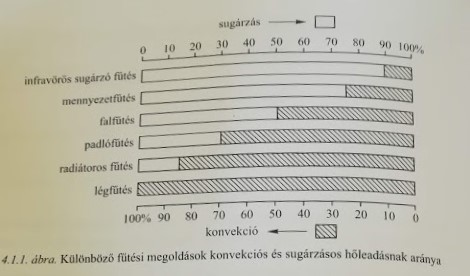
\includegraphics[width=8cm]{figures/konvrad}
%	\caption{Alacsony hőmérsékletű fűtés és magas hőmérsékletű hűtés c. könyv ábrája}
%		%\footnote{Jan Babiak, rehva Guidebook No.7}
%\end{figure}


%A levegő hőmérsékletére ezek a következőképp hatnak a leginkább:
%\begin{itemize}[noitemsep,topsep=0pt,parsep=0pt,partopsep=0pt]
%	\item a fűtőtestek konvektív és radiatív hőátadással is melegítik a környezetet
%	\item a radiatív energiát a tárgyak, falak nyelik el, amik ezáltal felmelegszenek (mintegy kapacitásként lesz egy hőtároló tömeg, ami a fűtés kikapcsolásával fenntartja a hőmérsékletet / lassítja a hűlést)
%	\item a fűtetlen falfelületek hűtik a szobát (külső hőmérséklet befolyása)
%\end{itemize}
%
%Így a kezdeti modellben azzal a feltételezéssel élek, hogy ezen kívül más hatás nem lép fel.
%
%A modellben feltételezem, hogy a fűtőtest felületi hőmérsékletével tudunk beavatkozni. A modellben paraméter a fűtőtestek hőátadási tényezője és felülete. Zavarásként (?) hat a külső hőmérséklet értéke, amit mérni is tudunk. Kimenet a belső hőmérséklet (térben konstansnak véve azt / átlagolva a szoba levegőjére)
%
%A modell felírásához a fűtőtest tulajdonságain kívül szükség van a szobában található levegő mennyiségére is. A zavarás hatását is fel kell írni, azaz hogy egy külső hőmérsékletváltozás hogyan jelenik meg a kimeneten. (Célszerű itt egy átviteli függvényt felírni először, szuperpozíciószerűen. A zavarás viszont nem a modell bemenetén és nem is a kimenetén hat.)

%A felírandó átviteli függvények:
%
%\begin{itemize}[noitemsep,topsep=0pt,parsep=0pt,partopsep=0pt]
%	\item levegő felmelegedése konstans külső hőmérsékletet feltételezve, fűtőtest egységugrással
%	\item levegő felmelegedése fűtés kikapcsolt állapota mellett, környezeti hőmérséklet ugrásával
%\end{itemize}
%
%Ezeket ráadtam a rendszerre és két bemenetű, egy kimenetű rendszerként identifikáltam.

%\pagebreak


%\subsubsection{Modellparaméterek}

%\subsection{-----}
%
%Fűtési típusok szerint:
%
%\begin{itemize}[noitemsep,topsep=0pt,parsep=0pt,partopsep=0pt]
%	\item radiátoros fűtés hőátvitele
%	\item padlófűtés hőátvitele
%\end{itemize}
%
%A fentiekre különböző értékű lesz a 
%
%\begin{itemize}[noitemsep,topsep=0pt,parsep=0pt,partopsep=0pt]
%	\item hőátadási tényező
%	\item hőtároló tömeg
%	\item költségfüggvény?
%	\item előremenő vízhőmérséklet és ezzel a leadott teljesítmény maximumértéke
%\end{itemize}
%
%ami így eltérő ház-modelleket fog eredményezni.


\pagebreak
\chapter{Helyiség modellje}\label{chap:helyiseg}

% Kiindulás ssc_house_heating_system

A szabályzótervezéshez rendelkezésre kell, hogy álljon a szabályzott szakasz modellje. Ezt két részre bontottam: először az épületszerkezet, azaz a helyiség modelljét írom fel, a fűtőtestekkel a \textit{\ref{chap:futotest}. fejezetben} foglalkozom. A \textit{\ref{fig:Simulink-minimalist}.~ábrán} látható a részekre bontott modell\footnote{A képen nyílt hurkú modell szerepel, a \textit{Vizsgálójelek} blokk jeleivel a fűtési rendszer tranziensei megfigyelhetők a \textit{Scope} ablakban.}, melyből a helyiség alrendszert tárgyalom ebben a fejezetben. Egy könnyen módosítható, koncentrált paraméterű hálózatot vettem fel, ahol minden elemhez lehet fizikai tartalmat rendelni. A szabályzótervezéshez a teljes modell gerjesztés-válasz kapcsolatára lesz majd szükségem.
%todo footnote

Az energetikai jellemzők az épület energetikai tanúsítványából kiolvashatók, így a modell paraméterezhető. A tervezési lépéseket a névleges modellre elvégezve a szabályzás rögtön működőképes, nincs szükség hosszas kalibrációs időszakra beüzemelésnél. A modellbeli eltéréseket később kompenzálni lehet, mérési adatok felhasználásával.% (historikus adatok felhasználásával). %A modellben a bizonytalanságok hatása adaptív szabályozással kezelhető (lesz).

\begin{figure}[H]
	\centering
	% trim={<left> <lower> <right> <upper>}
	%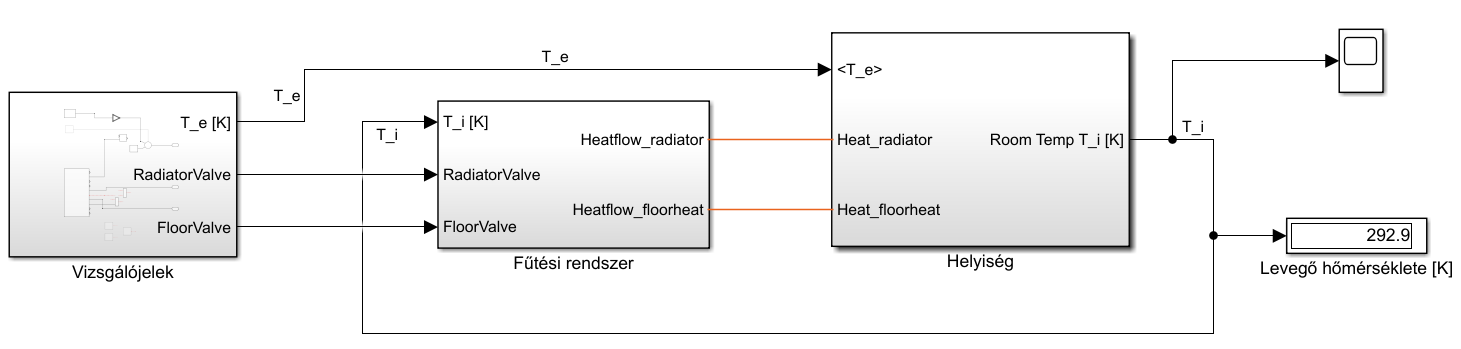
\includegraphics[trim=0 0 0 0, clip,width=\textwidth]{figures/simulink-network-minimalist-layout2}
	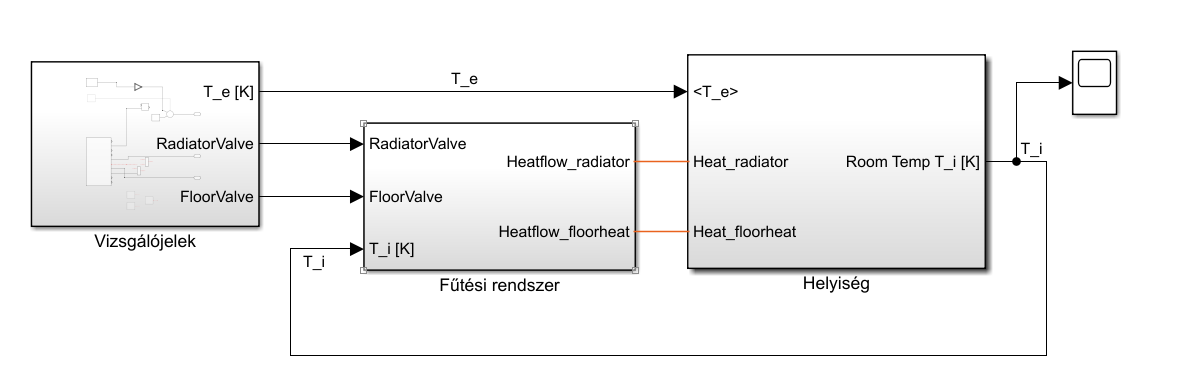
\includegraphics[trim=0 0 0 0, clip,width=\textwidth]{figures/simulink-network-minimalist-layout3}
	\caption{Fűtési rendszer modellje - fűtőtest és helyiség}
	\label{fig:Simulink-minimalist}
\end{figure}

\section{A modellalkotás folyamata}
%
%White-box
%grey-box
%black-box

% zavarás, bemenet, nem irányított bemenet

A gerjesztés-válasz kapcsolatot megkaphatjuk méréssel, szimulációval vagy egyenletek felírásával. Mindegyik módszernek van előnye és hátránya is:  ha a hatásmechanizmusok pontosan ismertek, használhatunk "white-box" modellt, amiben fizikai összefüggések szerepelnek. Ha a hatásmechanizmus nem ismert, fekete dobozként ("black-box") is kezelhetjük a rendszert, de az identifikációhoz nagyon sok mérésre van szükség, hogy a mérési hibákat és zavarásokat kiküszöbölhessük.%\cite{THIEBLEMONT2017485}

Én a fizikai modell felírását választottam, melynek dinamikáját megvizsgálom a szabályozótervezéshez. Megfelelő gerjesztő jelekkel identifikálva előáll a modell átviteli függvénye (\textit{\ref{chap:ident}. fejezet}). Ehhez sokkal egyszerűbb eljutni, mint mérésekkel, mivel a Simulinkben megvalósított hálózatra az identifikáció sokkal egyszerűbb, mint valós rendszerre. A vizsgálójelek tetszőlegesen megválaszthatók, például a külső hőmérséklet hatása is pontosan meghatározható a \textit{\ref{fig:Simulink-minimalist}. ábrán} látható elrendezésben\footnote{Az átláthatóság kedvéért csak a kimenetet kötöttem rá a scope-ra, de a szimuláció közben az összes bemenetet, illetve belső változók állapotát is nyomon követhetjük}. A helyiség egy MISO (több bemenetű, egy kimenetű) rendszer, terepi méréseket használva csak hosszas mérésekből lehet szétválasztani a bemenetek (fűtés, külső hőmérséklet, napsütés) hatását a belső hőmérsékletre.



%Ha később páratartalom szabályzása is szóba kerül, még bonyolultabb a helyzet.


%\cite{SCHIRRER201686}

% --------------------------- kihúzva:
%A szakirodalomban pl. \cite{THIEBLEMONT2017485} és \cite{SCHIRRER201686} érinti ezt a kérdést:
%
%A szabályzótervezés során néhányan egyáltalán nem alkotnak modellt, csak a mért adatokat használják fel, ami eléggé időigényes: az identifikációhoz egy megfelelően nagy amplitúdójú vizsgálójelre van szükség. Viszont egy 10\si{\celsius}-kal felfűteni egy helyiséget hosszú ideig tart, ami alatt biztosan meg fog változni pl. a külső hőmérséklet. Ha a mérésekben a különböző inputok hatása a kimeneten nem különíthető el jó, az identifikáció nehéz lesz. Illetve külső hőmérséklet sem változik ugrásszerűen, a lassú időbeli változás \textit{nem jó vizsgálójel} identifikációhoz.
% ---------------------------

%Lényegében én is mért adatokat használok NEMMM, EZÉRT VAN A TANÚSÍTVÁNY!, tulajdonképpen, mivel a modellt olyan alakban kéne felírni, hogy a szabályzó azt futtatni tudja. (?)


% ---------------------------


%Vizsgálójel kiválasztása
%
%Modell struktúra kiválasztása - átviteli függvények pólusainak, zérusainak száma
%
%
%Viszont az ident toolbox tf identjénél kihasználtam azt, hogy a rendszer jellegét ismerem, azaz hogy hány pólusa és hány zérusa van a szakasznak  / felnyitott körnek. Így lett egy nagyon jól illeszkedő átviteli függvényem.
%
%Én összeraktam a fizikai modellt simulinkben (ez white-box) majd annak az ugrásválaszát mértem. Így nem egy állapotteres modell, hanem egy átviteli fv. "keletkezett".


Helyiségenkénti hőmérséklet-szabályzás esetén a belső hőmérsékletre adott egy referencia és egy mért érték.
Helyiségenként számos olyan tényező figyelembe vehető, melyek a teljes épületre különbözőek: a helyiség tájolása, az ablakok mérete, a felhasználás módja mind jobban kezelhető helyben, mint egy központi irányítással. Ezek mind-mind zavarásnak számítanak, ha pedig egy-egy helyiség hőmérsékletét mérjük, a zavarások ellenében ott tudunk beavatkozni, ahol azok hatnak. A helyi szabályozás referenciajeleit a lakók, dolgozók komfortérzetének megfelelően kell megadni.

A helyiség levegőjének hőmérsékletét mindenhol ugyanakkorának (homogénnek) feltételezem. A szabályzás a helyiség hőveszteségét egyenlíti ki, amit az alacsonyabb külső hőmérséklet okoz. Nem foglalkozok például szellőzésből, helyiségek közti hőmérséklet-különbségből\footnote{A modellezés egyszerűsítése végett több helyiség egymásra hatását nem veszem figyelembe.}, vagy emberek jelenlétéből származó belső zavarással.

A fűtést padlófűtés és radiátor biztosítja, mindkettőben szeleppel szabályozható az átfolyó vízmennyiség.

\section{A Simscape termikus elemei}

A \textit{\ref{fig:Simscape}. ábrán} látható egy termikus mintahálózat, mellyel bemutatom a Simscape csomag elemeit, melyből a helyiség modellje is felépíthető.

A források lehetnek fix hőmérsékletű elemek (feszültségforrás) illetve hőáram forrásai (áramforrás).
%A hasonlóság nem véletlen a villamos hálózatokkal. Felfedezhető, hogy a hőáramot a hőmérséklet-különbség hozza létre, nagysága pedig fordítottan arányos a hővezetési tényezővel. 
A "vezetékek" így azonos hőmérsékletű (ekvipotenciális) pontokat kötnek össze, ezekre hőmérsékletmérőket helyezhetünk. A különböző elemekkel sorba kapcsolva helyezhetők el hőáramlást mérő blokkok.

A hőáramlást a hőellenállások korlátozzák, mivel azokon hőmérsékletesés mérhető. (Az ábrán mért hőáram a hőellenálláson eső hőmérséklettel arányos, a \textit{\ref{eq_hoaram_alap}. egyenlet} szerint.) A hőtároló elemeknek tömege és fajhője megadja a hőkapacitásukat, így ezek feltöltődhetnek, energiát tárolhatnak.


A mintahálózat egy RC-tagnak felel meg, erre a szabályzótervezés lépései a következők lennének:%\footnote{Tekintsük a mintahálózatot és az itt részletezett lépéseket egy szemléletes példának, ugyanis a szakdolgozatban tárgyalt hálózatra is ezeken a lépéseken fogok végighaladni.}:

Az identifikációnál ismert a rendszer jellege, így 0 zérussal, 1 pólussal átviteli függvényt identifikálnék.
Erre szabályzót lehetne tervezni. A szimuláció során a termikus hálózat alapjele helyére kerülne a szabályzó beavatkozó jele. A visszacsatolás a hőmérő kimenetéről történne. Ekkor, mivel a tervezés során használt modell és a  szakasz között nincs eltérés (angolul \textit{mismatch}), a szabályzás jól működik.
A paraméterek módosításával a szabályzó robusztusságát lehet tesztelni.

Ha ez a hálózat egy tényleges fizikai rendszer (például egy vízforraló) modellje lenne, akkor a szabályzás történhetne úgy, hogy a szabályzó egy beágyazott számítógépen fut, majd a teljesítményelektronikán keresztül a kívánt teljesítményt szolgáltatja, hogy például azonos hőmérsékleten tartsa benne a teát.

\begin{figure}[H]
	\begin{subfigure}[t]{\textwidth}
		\centering
		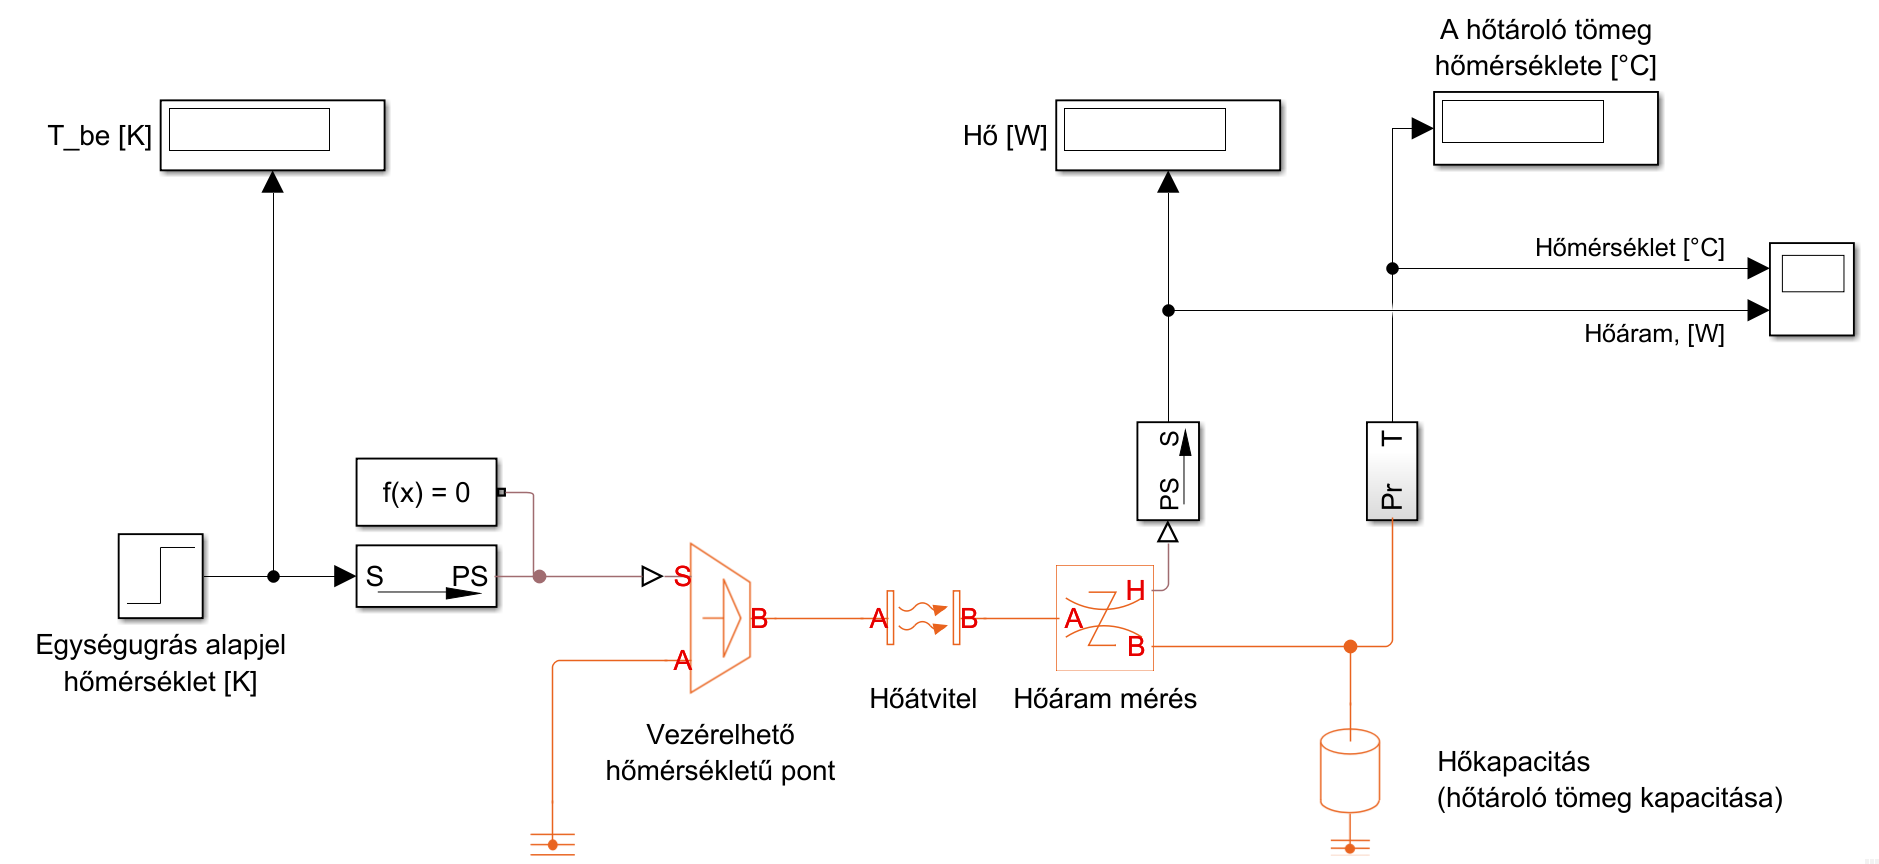
\includegraphics[width=\textwidth]{figures/SimscapeGeneral}
		\caption{Simscape termikus modell}
		\label{fig:SimscapeGeneral}
	\end{subfigure}%
	\smallskip
	\vspace*{10pt}
	\begin{subfigure}[t]{\textwidth}
		\centering
		% trim={<left> <lower> <right> <upper>}
		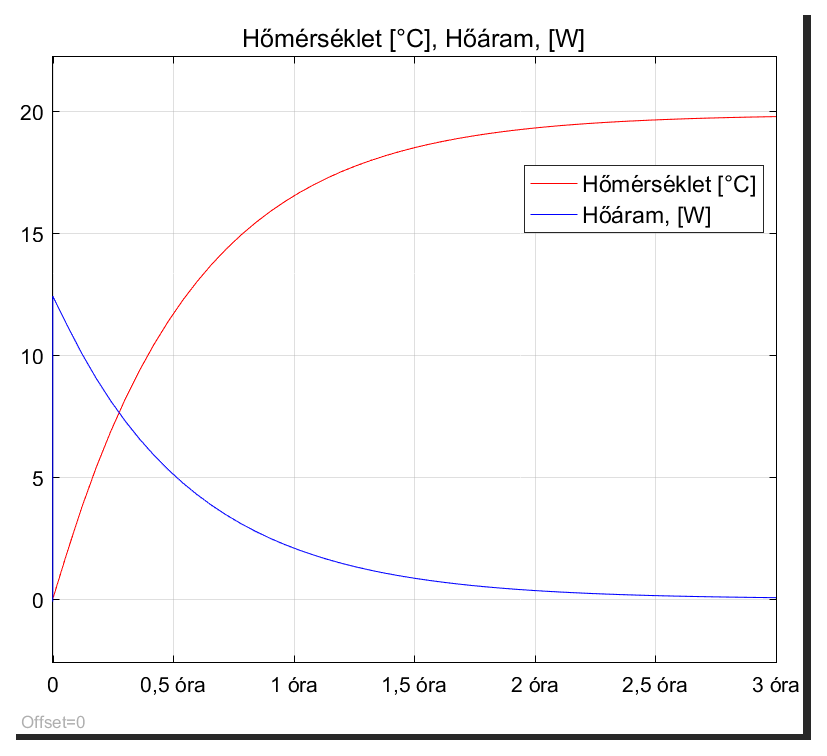
\includegraphics[trim=2 12 5 0, clip,width=0.49\textwidth]{figures/step_Simscape}
		\caption{Modell ugrásválasza}
		\label{fig:SimscapeStep}
	\end{subfigure}
	%	~
	%	\begin{subfigure}[t]{0.49\textwidth}
	%		\centering
	%%		\includegraphics[height=1.9in]{SSy}
	%%		\caption{Szimulált ugrásválasz}
	%%		\label{fig:SSy}
	%	\end{subfigure}	
	\caption{Tranziens (instacioner) hőtranszfer modellezése}
	\label{fig:Simscape}
	\centering
\end{figure}


%Természetesen lehetett volna nagyon sok állapotú állapoteres modellt is létrehozni, ám rengeteg nem mérhető belső változója lett volna, emiatt nem biztos hogy teljesen irányítható vagy megfigyelhető rendszert kaptam volna, így pedig a szabályzótervezés nem működik.


 
% \textbf{ÁBRA WHITE-BOX MODELRŐL, ÉS BLACKBOX IDENTIFIKÁCIÓRÓL. ILLETVE WHITEBOX IDENT.}


\section{Épületfizikai alapösszefüggések}
 
 A fizikai modell felírásához szükség van néhány alapösszefüggésre.
 %TODO ide még valami bevezető
 
 \subsubsection*{Hőátbocsátási tényező számítása}
 %TODO mi ez és miért jó
 A hőátadási tényező a levegő és egy felület közötti hőátadást mutatja meg,
 a rétegrendi hőátbocsátási tényező pedig számba veszi az összes réteg hatását: fal esetén annak két oldalán található levegő hőmérséklet-különbségével arányos hőáramot adja meg. 
 
 \begin{equation}\label{eq_hoatbcsatas_U}
 \begin{aligned}
 U = \frac{1}{\frac{1}{\alpha_e}+\sum\limits_{i}^{}\frac{d_i}{\lambda_i}+\frac{1}{\alpha_i}}
 \end{aligned}
 \end{equation}
 
\subsubsection*{Hővezetés, hőáramlás, hősugárzás}

A hőátadásnak három fajtája van, ezek 

\begin{equation} \label{eq_hoaram_alap}
\begin{aligned}
q = U\Delta t = \frac{\Delta t}{R}
\end{aligned}
\end{equation}

Ahol 

\begin{itemize}[itemsep=6pt,topsep=0pt,parsep=0pt,partopsep=0pt]
	\item[] $q$ a hőáram [\si[per-mode=fraction]{\watt\per\metre\squared}]
	\item[] $\Delta t$ a hőmérséklet-különbség (a potenciálkülönbség analógiájára)
	\item[] $U$ a hővezetési tényező [\si[per-mode=fraction]{\watt\per\metre\squared\per\kelvin}], reciproka az $R$ hővezetési ellenállás.
\end{itemize}


A külső falon a hőáramsűrűség:

\begin{equation}\label{eq_hoveszteseg}
\begin{aligned}
q &= U_{fal}\Delta t = \alpha_i\left(t_i-t_{i,fal}\right)
\end{aligned}
\end{equation}

Az U hőátbocsátási tényező szerepe tehát az, hogy a rétegek hatását együttesen kezelhessük. A \ref{table_house_parameters} táblázatban szerepel mindkét féle hőátadási tényező. 



\begin{table}[H]
	\footnotesize
	\centering
	\caption{Hőközlés fajtái}
	%\renewcommand{\arraystretch}{2} % to increase cell height
	%\taburulecolor{gray}
	%\begin{tabular}{|p{0.8cm}|p{1cm}|p{1cm}|p{1cm}|p{1cm}|p{1cm}|p{1cm}|p{1cm}|}
	%
	\newcolumntype{C}[1]{>{\centering\arraybackslash}p{#1}}
\newcolumntype{R}[1]{>{\raggedleft\arraybackslash}p{#1}}


\begin{tabu}{p{1.5cm}C{1.6cm}C{7cm}C{4cm}}
	%{p{1.5cm}|C{0.8cm}|C{0.8cm}|C{0.8cm}|C{0.8cm}|C{0.8cm}|C{0.8cm}|C{0.8cm}|C{0.8cm}|}
	%\multicolumn{1}{l}{}&\multicolumn{8}{l}{SDO header (első adatbyte) - master kérése}
	%\\ 		\cline{2-9}\cline{2-9}
	\hline
	\\
	& együtthatója &  a hőátadás szereplői & példa
	\\
	konvektív &  $\lambda$& áramló közeg -- szilárd anyag felülete & levegő vagy víz áramlása
	\\
	konduktív &  $h_c$&  az anyag molekulái között & az anyag belsejében
	\\
	radiatív &  $h_r$& tárgyak között, felszínükkel arányosan & hősugárzás 
	\\
%	& méret & $h_t$, átlag    & hőtároló tömeg & hőkapac
%	\\
%	& méret & $h_t$, átlag    & hőtároló tömeg & hőkapac
%	\\
%	& méret & $h_t$, átlag    & hőtároló tömeg & hőkapac
%	\\
%	& méret & $h_t$, átlag    & hőtároló tömeg & hőkapac
%	\\
%	& méret & $h_t$, átlag    & hőtároló tömeg & hőkapac
%	\\ %\hline
%	külső fal & 4.5 \si{\metre\squared} & 2 \si[per-mode=fraction]{\watt\per\metre\squared\per\kelvin} & 900kg & 756 \si[per-mode=fraction]{\kilo\joule\per\kelvin}
%	\\ %\hline
%	ablak & 4 \si{\metre\squared} & 4 \si[per-mode=fraction]{\watt\per\metre\squared\per\kelvin} & 0 & 0
%	\\ %\hline
%	belső válaszfalak & 50 \si{\metre\squared} & 7 \si[per-mode=fraction]{\watt\per\metre\squared\per\kelvin} & 5000kg & 4.2 \si[per-mode=fraction]{\mega\joule\per\kelvin}	
%	\\ %\hline
%	padló & 16 \si{\metre\squared} & 11 \si[per-mode=fraction]{\watt\per\metre\squared\per\kelvin}  & 3200kg &2.7 \si[per-mode=fraction]{\mega\joule\per\kelvin}
%	\\ %\hline
%	mennyezet & 16 \si{\metre\squared} & 5 \si[per-mode=fraction]{\watt\per\metre\squared\per\kelvin} & 3200kg &2.7 \si[per-mode=fraction]{\mega\joule\per\kelvin}	
	\\ \hline

%	belső válaszfalak & 50 \si{\metre\squared} & 7 & 50*100kg & 50*100*840		
%	\\ \hline
%	11 & Internal limit active
%	\\ \hline
%	12-13 & Operation mode specific
%	\\ \hline
%	14-15 & Reserved
\end{tabu}

	\label{tab:HeatExchangeTypes}
	%
	%\label{tab:TabularExample}
	%\tabref{TabularExample}~táblázat
\end{table}

\subsubsection*{Hőtároló képesség}


Falszerkezeteknél annak hőtároló képessége adja meg, hogy \SI{1}{\celsius}-os hőmérséklet-változás esetén mennyivel változik a szerkezet energiája.

Az \textit{EN ISO 13790} szerint az épület hőtároló tömege az épület belső levegőjével közvetlen kapcsolatban lévő határolószerkezetek hőtároló tömegének összege.

\begin{equation}\label{eq_hotarolo-tomeg}
\begin{aligned}
M= \rho d A\\[10pt]
\Delta Q= cM\Delta t
\end{aligned}
\end{equation}

Ebben az esetben eltérek a szabványban használt módszerektől. Az \textit{MSZ 24140} megadja, hogy egyes anyagoknál mekkora réteget kell figyelembe venni egy napos ciklusidejű hőtárolásra. Ez azért nem pontos, mert több napos átmelegedési időkkel nem számol. Az energetikai tanúsítványok azonban tartalmazzák a teljes tömeget és a szabvány szerinti hőtároló tömeget is. A modellben a teljes tömeg szerepel.




\begin{table}[H]
	\footnotesize
	\centering
	\caption{Jelölések}
	%\renewcommand{\arraystretch}{2} % to increase cell height
	%\taburulecolor{gray}
	%\begin{tabular}{|p{0.8cm}|p{1cm}|p{1cm}|p{1cm}|p{1cm}|p{1cm}|p{1cm}|p{1cm}|}
	%
	\newcolumntype{C}[1]{>{\centering\arraybackslash}p{#1}}
\newcolumntype{R}[1]{>{\raggedleft\arraybackslash}p{#1}}

\setstretch{1.8}

\begin{tabulary}{\linewidth}{LLc}
	%\begin{tabulary}{|p{3cm}|p{1.2cm}|p{2cm}|p{3cm}|p{3cm}|}
	%{p{1.5cm}|C{0.8cm}|C{0.8cm}|C{0.8cm}|C{0.8cm}|C{0.8cm}|C{0.8cm}|C{0.8cm}|C{0.8cm}|}
	%\multicolumn{1}{l}{}&\multicolumn{8}{l}{SDO header (első adatbyte) - master kérése}
	%\\ 		\cline{2-9}\cline{2-9}
	\hline
	${Q}_{total} $& hőáram 				& \si[per-mode=fraction]{\watt} = \si[per-mode=fraction]{\joule\per\second}
	\\
	$A $		& felszín				& \si[per-mode=fraction]{\watt\per\metre\squared}
	\\
	$U$ 		& réteges szerkezet hőátbocsátási tényezője  & \si[per-mode=fraction]{\watt\per\metre\squared\per\kelvin}
	\\
	$q_{total} $& teljes hőáramsűrűség 	& \si[per-mode=fraction]{\watt\per\metre\squared}
	\\
	$h_{total}$	& teljes hőcsere együttható & \si[per-mode=fraction]{\watt\per\metre\squared\per\kelvin}
	\\
	$h_{r}$ 	& radiatív hőátadási tényező & \si[per-mode=fraction]{\watt\per\metre\squared\per\kelvin}
	\\
	$h_{c}$, $\alpha$
				& konvektív hőátadási tényező
										& \si[per-mode=fraction]{\watt\per\metre\squared\per\kelvin}
	\\
	$\lambda$  	& konduktív hőátadási tényező & \si[per-mode=fraction]{\watt\per\metre\squared\per\kelvin}
	\\
	$\varepsilon$
				& emisszivitás & --
	\\
	$t_{ref}$ 	& referencia hőmérséklet& \si[per-mode=fraction]{\celsius}
	\\
	$t_i$ 		& belső hőmérséklet 	& \si[per-mode=fraction]{\celsius}
	\\
	$t_e$ 		& külső hőmérséklet 	& \si[per-mode=fraction]{\celsius}
	\\
	$c$ 		& fajhő 		& \si[per-mode=fraction]{\joule\per\kilogram\per\kelvin}
	\\
	$C$		& hőkapacitás 		& \si[per-mode=fraction]{\joule\per\kelvin}
	\\
	$\dot{m}$ 	& tömegáram 	& \si[per-mode=fraction]{\kilogram\per\second}
	\\
	$\xi$, $u_1,u_2$
				& szelep kinyitásának mértéke [0..1]				& $\%$
	\\
	$\Delta t_m$& közepes hőmérsékletkülönbség 	& \si[per-mode=fraction]{\celsius}
	\\
	$t_i$ 		& belső hőmérséklet 	& \si[per-mode=fraction]{\celsius}

%	& méret & $h_t$, átlag    & hőtároló tömeg & hőkapac
%	\\
%	& méret & $h_t$, átlag    & hőtároló tömeg & hőkapac
%	\\
%	& méret & $h_t$, átlag    & hőtároló tömeg & hőkapac
%	\\
%	& méret & $h_t$, átlag    & hőtároló tömeg & hőkapac
%	\\
%	& méret & $h_t$, átlag    & hőtároló tömeg & hőkapac
%	\\ %\hline



%	külső fal & 4.5 \si{\metre\squared} & 2 \si[per-mode=fraction]{\watt\per\metre\squared\per\kelvin} & 900kg & 756 \si[per-mode=fraction]{\kilo\joule\per\kelvin}
%	\\ %\hline
%	ablak & 4 \si{\metre\squared} & 4 \si[per-mode=fraction]{\watt\per\metre\squared\per\kelvin} & 0 & 0
%	\\ %\hline
%	belső válaszfalak & 50 \si{\metre\squared} & 7 \si[per-mode=fraction]{\watt\per\metre\squared\per\kelvin} & 5000kg & 4.2 \si[per-mode=fraction]{\mega\joule\per\kelvin}	
%	\\ %\hline
%	padló & 16 \si{\metre\squared} & 11 \si[per-mode=fraction]{\watt\per\metre\squared\per\kelvin}  & 3200kg &2.7 \si[per-mode=fraction]{\mega\joule\per\kelvin}
%	\\ %\hline
%	mennyezet & 16 \si{\metre\squared} & 5 \si[per-mode=fraction]{\watt\per\metre\squared\per\kelvin} & 3200kg &2.7 \si[per-mode=fraction]{\mega\joule\per\kelvin}	
	\\ \hline
%	belső válaszfalak & 50 \si{\metre\squared} & 7 & 50*100kg & 50*100*840		
%	\\ \hline
%	11 & Internal limit active
%	\\ \hline
%	12-13 & Operation mode specific
%	\\ \hline
%	14-15 & Reserved
\end{tabulary}

	\label{tab:Nomenclature}
	%
	%\label{tab:TabularExample}
	%\tabref{TabularExample}~táblázat
\end{table}

\section{A megvalósított modell}

Figyelembe kell vennem a ház hőveszteségeit és hőtároló képességét is, a () és () egyenletek alapján, melynek paraméterei a \ref{table_house_parameters}. táblázatban találhatók.
%Ennek paraméterei: a határoló elemek felszíne, hőátbocsátási tényezője, a hőtároló elemek fajhője.
Az alábbi táblázat értékeinek nagy részét ki lehet tölteni a tanúsítványból. Feltételezem, hogy ez rendelkezésre áll, hiszen ennek elkészítésére elég sok esetben szükség van (adásvétel, felújítás, stb.).
Az épület éves hőigénye numerikusan is szerepel a tanúsítványban. Itt a fűtési rendszer tulajdonságain kívül a várható napsütéses órák számát és a használati melegvíz előállításának energiaigényét figyelembe veszi\footnote{A hőigény számításához törvényi előírások alapján különböző korrekciós tényezőket használnak.}.
%TODO hol van ez a törvényben?

A Matlab Simscape model és \textit{Lapusan} \cite{LAPUSAN2016320}
%\footnote{Development of a Multi-Room Building Thermodynamic Model Using Simscape Library - Ciprian Lapusan}
 hőátadásnál a réteges szerkezetekben számolt konvekcióval és kondukcióval is. Viszont ezek az adatok egyben is kezelhetők, a követelményeket ezekre a költségoptimalizált követelményszint\footnote{ A  költségoptimalizált követelményszintek megtalálhatók a 7/2006. rendelet \cite{TNM2006} 5. mellékletében.} adja meg. Régebbi épületek ezt a szintet nem tudják teljesíteni, ezekre jellemző értékeket adtam meg az alábbi táblázatban. 
%todo táblázat

Ám nem szabad összekeverni az U értéket (rétegrendi hőátbocsátási tényező) és az $\alpha_i$ konvektív hőátadási tényezőt, amit a válaszfalakra, padlóra és mennyezetre adtam meg, hiszen ezeken a modell szerint a helyiség nem veszt hőt, csak a hőtároló elemeknek adódik át.
%todo kell-e ez itt. A hőátadási tényező a levegő és egy felület közötti hőátadást mutatja meg, a rétegrendi hőátbocsátási tényező pedig számba veszi az összes réteg hatását: fal esetén annak két oldalán található levegő hőmérséklet-különbségével arányos hőáramot adja meg.

%TODO clarify - Viszont itt célszerű lenne a konvektív hőátadást is beleszámolni. 


%(Baromi érdekes, hogy nálunk otthon van egy hőcserélő a használati melegvíz és a fűtési rendszer között, annak a hatásait is lehetne nézni.)

%\begin{table}[ht]
%	\footnotesize
%	\centering
%	\caption{Az órajel-generátor chip órajel-kimenetei.} \label{tab:SysClocks}
%	\begin{tabular}{ | l | c | c |}
%		\hline
%		Órajel & Frekvencia & Cél pin \\ \hline
%		CLKA & 100 MHz & FPGA CLK0\\
%		CLKB & 48 MHz  & FPGA CLK1\\
%		CLKC & 20 MHz  & Processzor\\
%		CLKD & 25 MHz  & Ethernet chip \\
%		CLKE & 72 MHz  & FPGA CLK2\\
%		XBUF & 20 MHz  & FPGA CLK3\\
%		\hline
%	\end{tabular}
%	\label{tab:TabularExample}
%\end{table}






 A példában a Schönherz Zoltán Kollégium egy szobájának megfelelő méretű helyiséget vettem fel. Minden szobának van ablaka és külső fala, egy átlagos szobát 4 másik vesz körül. A belső falakon nem veszt hőt, csak az ablakon ill. a külső falon. Feltételezzük, hogy a radiátoros fűtést egy szeleppel szabályozhatjuk, amit tetszőleges mértékben nyithatunk ki.
 A napsütés hőnyereségét is figyelembe vehetjük.%, úgy, hogy egy hőforrás a padlót melegíti.

\section{A modell}
\begin{figure}[H]
	\centering
	% trim={<left> <lower> <right> <upper>}
	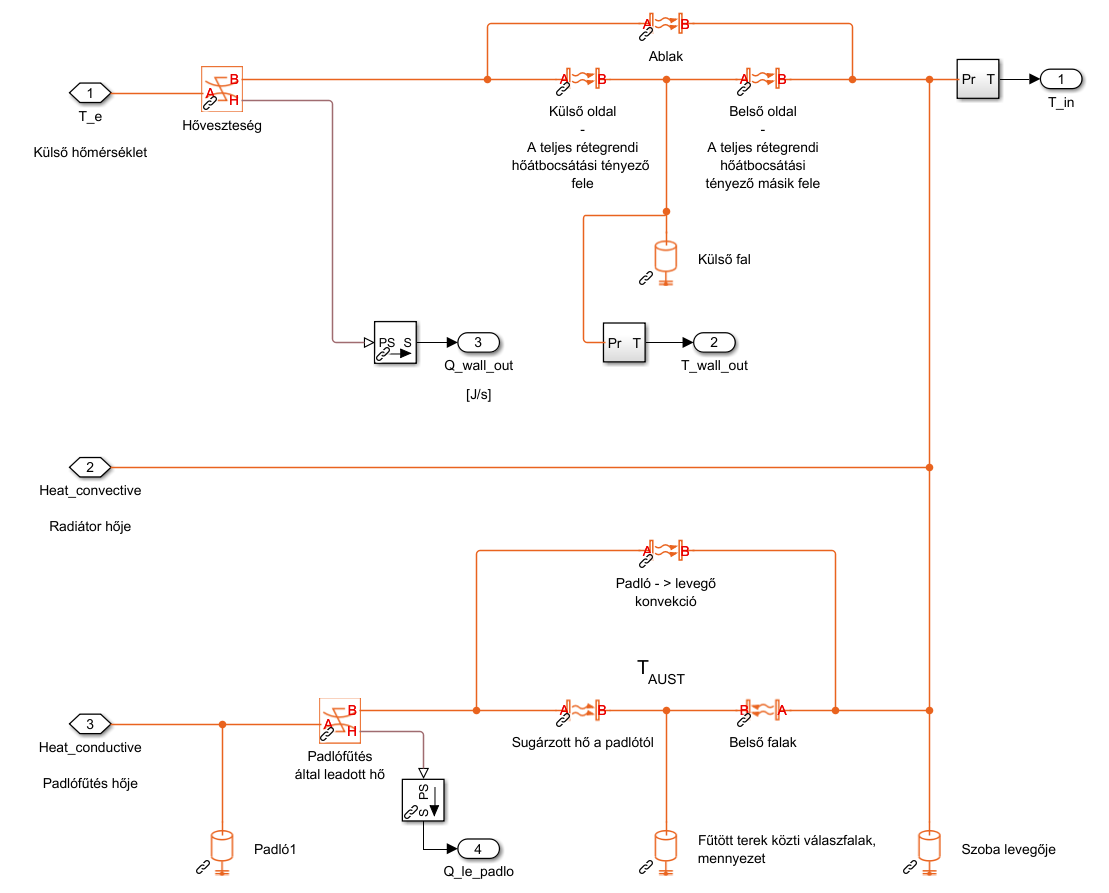
\includegraphics[trim=0 12 5 0, clip,width=\textwidth]{figures/SimscapeHouse}
	\caption{Helyiség termikus modellje}
	\label{fig:SimscapeHouse}
\end{figure}

A helyiség modellje a \textit{\ref{fig:SimscapeHouse}. ábrán} látható, három bemenete van: külső hőmérséklet, radiátor hője és a padlófűtés hője.
A külső hőmérséklet egy \say{feszültség jellegű} bemenet, hőáramot nem szab meg.
A radiátor \say{áram jellegű} kimenetet ad, hiszen itt a képlet a leadott hőt számítja: a radiátor konduktív hőárama közvetlenül a levegőt melegíti. A padlófűtés először a padlónak adja át a hőt, utána pedig a levegőnek (konduktív hőátadás), illetve a falaknak (sugárzó, radiatív hőátadás).

A levegőnek, padlónak, falaknak tömegüknél és fajhőjüknél fogva mind-mind van egy hőtároló képességük (\textit{\ref{table_house_parameters}. táblázat}), egy bizonyos idő alatt tudnak feltöltődni vagy hőenergiájukat leadni: hőmérsékletük nem változhat ugrásszerűen. %Mindezekben villamosmérnöki szemszögből felfedezhetjük az analógiát a villamos hálózatokkal.


\begin{table}[H]
	\footnotesize
	\centering
	\caption{A helyiség hőveszteséget okozó elemei}
	\renewcommand{\arraystretch}{1.3} % to increase cell height
	\taburulecolor{gray}
	%\begin{tabular}{|p{0.8cm}|p{1cm}|p{1cm}|p{1cm}|p{1cm}|p{1cm}|p{1cm}|p{1cm}|}
	\newcolumntype{C}[1]{>{\centering\arraybackslash}p{#1}}
\newcolumntype{R}[1]{>{\raggedleft\arraybackslash}p{#1}}
\begin{tabu}{@{}p{3.5cm}p{1.2cm}p{2cm}p{3cm}p{3cm}@{}}
	%\begin{tabu}{|p{3cm}|p{1.2cm}|p{2cm}|p{3cm}|p{3cm}|}
	%{p{1.5cm}|C{0.8cm}|C{0.8cm}|C{0.8cm}|C{0.8cm}|C{0.8cm}|C{0.8cm}|C{0.8cm}|C{0.8cm}|}
	%\multicolumn{1}{l}{}&\multicolumn{8}{l}{SDO header (első adatbyte) - master kérése}
	%\\ 		\cline{2-9}\cline{2-9}
	veszteséges elemek& méret & $U$    & hőtároló tömeg & hőkapacitás
	\\ \hline%\hhline{=====}
	külső fal & 4.5 \si{\metre\squared} & 2 \si[per-mode=fraction]{\watt\per\metre\squared\per\kelvin} & 900kg & 756 \si[per-mode=fraction]{\kilo\joule\per\kelvin}
	\\ %\hline
	ablak & 4 \si{\metre\squared} & 4 \si[per-mode=fraction]{\watt\per\metre\squared\per\kelvin} & - & -
	\\ %\hline
\end{tabu}

%	\begin{subtable}
%		\newcolumntype{C}[1]{>{\centering\arraybackslash}p{#1}}
\newcolumntype{R}[1]{>{\raggedleft\arraybackslash}p{#1}}


\begin{tabu}{@{}p{3.5cm}p{1.2cm}p{2cm}p{3cm}p{3cm}@{}}
	csak hőtároló elemek & méret & $h_t$    & hőtároló tömeg & hőkapacitás \\	\hline%\hhline{=====}
	belső válaszfalak & 50 \si{\metre\squared} & 7 \si[per-mode=fraction]{\watt\per\metre\squared\per\kelvin} & 5000kg & 4.2 \si[per-mode=fraction]{\mega\joule\per\kelvin}	
	\\ %\hline
	padló & 16 \si{\metre\squared} & 11 \si[per-mode=fraction]{\watt\per\metre\squared\per\kelvin}  & 3200kg &2.7 \si[per-mode=fraction]{\mega\joule\per\kelvin}
	\\ %\hline
	mennyezet & 16 \si{\metre\squared} & 5 \si[per-mode=fraction]{\watt\per\metre\squared\per\kelvin} & 3200kg &2.7 \si[per-mode=fraction]{\mega\joule\per\kelvin}	
	\\ %\hline
\end{tabu}

%	\end{subtable}
	\label{table_house_parameters}
	%\label{tab:TabularExample}
	%\tabref{TabularExample}~táblázat
\end{table}

\begin{table}[H]
	\footnotesize
	\centering
	\caption{A helyiség veszteségmentes elemei}
	\renewcommand{\arraystretch}{1.3} % to increase cell height
	\taburulecolor{gray}
	\newcolumntype{C}[1]{>{\centering\arraybackslash}p{#1}}
\newcolumntype{R}[1]{>{\raggedleft\arraybackslash}p{#1}}


\begin{tabu}{@{}p{3.5cm}p{1.2cm}p{2cm}p{3cm}p{3cm}@{}}
	csak hőtároló elemek & méret & $h_t$    & hőtároló tömeg & hőkapacitás \\	\hline%\hhline{=====}
	belső válaszfalak & 50 \si{\metre\squared} & 7 \si[per-mode=fraction]{\watt\per\metre\squared\per\kelvin} & 5000kg & 4.2 \si[per-mode=fraction]{\mega\joule\per\kelvin}	
	\\ %\hline
	padló & 16 \si{\metre\squared} & 11 \si[per-mode=fraction]{\watt\per\metre\squared\per\kelvin}  & 3200kg &2.7 \si[per-mode=fraction]{\mega\joule\per\kelvin}
	\\ %\hline
	mennyezet & 16 \si{\metre\squared} & 5 \si[per-mode=fraction]{\watt\per\metre\squared\per\kelvin} & 3200kg &2.7 \si[per-mode=fraction]{\mega\joule\per\kelvin}	
	\\ %\hline
\end{tabu}

	\label{table_house_parametersB}
\end{table}


%A modell mintavételi ideje?
%A teljesítményeket megnöveljük és semmi mást, az nem lesz ekvivalens. 

\subsubsection*{Hőigény:}

A külső falon

\begin{equation}\label{eq_hoigeny}
\begin{aligned}
		Q_{ki,fal} &= U_{fal}A_{fal}\Delta T = 200\si{\watt}\\[10pt]
		Q_{ki,ablak} &= U_{ablak}A_{ablak}\Delta T = 400\si{\watt}
\end{aligned}
\end{equation}

Amennyiben a méretezési hőmérséklet $\Delta T=$ \SI{-2}{\celsius}, ami a téli átlaghőmérséklet Magyarországon.
%TODO honnan \footnote{Épületfizika kurzus alapján vettem az átlaghőmérsékletet \SI{-2}{\celsius}-nak.}


%(Gondolatkísérlet: HA nem hatna zavarás, csak az időállandók számítanának, a pontos teljesítményveszteségek, nyereségek nem. Azaz mindegy volna hogy 1000W hő szökik ki és ehhez tartozik 1500W-nyi fűtési kapacitás, vagy hogy 5000W és 7500W ezek az értékek. Ám pl. napsütés hatásakor nem csak az arányok hanem a konkrét teljesítmények is kellenek...

%Így a modell egyik belső változója bizonyosan a teljesítmény kell, hogy legyen. Erre a belső változóra hat majd zavarás: emberek jelenléte kb. \SI{80}{\watt} 1 főre, napsütés, szellőztetés, stb.)

%\hrulefill


%Erre ki kellene számítani a hőigényt, figyelembe véve azt hogy mennyi hő szökik el a külső és belső határoló felületeken keresztül.
%A gyakorlati alkalmazásokban szeretnék majd az energetikai tanúsítványból kiindulni.%, így gyakorlatilag a szoba energetikai tanúsítását végzem el - olyan szinten, amennyire nekem szükséges.


%Ashrae HVAC - 6.19 Panel H \& C. - Controls strategy
%
%A modellt a jellemző szerkezeti tulajdonságok alapján írtam fel (indoklás a táblázathoz). A modellezés Gouda alapján történik, gyakorlatilag csomóponti egyenleteket kell felírni az alábbi hálózatra, amiben az ellenállások a rétegrendi hőátbocsátási tényező reciprokai. A hőtároló képességeket kapacitások modellezik. Ezeket az elemeket Simscape-ben implementáltam, a hőáramok így áttekinthetők és a paraméterek könnyen változtathatók.
%
%A ház modelljének felírásakor figyelembe vettem a hőtároló elemeket. A pontos (reális) modell felállításakor ezek hőtartalmát (a hőáram integrálja egyensúlyi állapotban legyen 0, azaz egy nagyobb ciklusban a felvett és leadott hője egyenlő) az egyensúlyi állapothoz közelinek vettem.
%
%Viszont a szabályzótervezéshez identifikálni kell, ekkor pedig a falak, ill. szoba levegőjének kezdeti állapotát (hőmérsékletét) azonosnak vettem a külső hőmérséklettel. Így ha a hőkülönbség a modell kimenő jele, akkor lineáris a rendszer: 0 bemenetre (fűtés) 0 kimenetet ad.

%\subsection{Megvalósítás MATLAB-ban}

%a simscape elemek kapcsolatai

\section{Fűtési rendszer és ház kapcsolata}

\begin{formal}
	\textbf{Megjegyzés:}
	Ha a szabályzást egy már meglévő épületre tervezzük, akkor csak a rendszerek adatait kell felvenni, illetve identifikálni. A szakdolgozatban tárgyalt egyszerű példa során csak egy részét ismerem a paramétereknek, tehát méretezési kérdéseket is fogok érinteni.  Szerencsére az új építésű házaknál kötelező energetikai tanúsítás%\footnote{A rendelet \cite{TNM2006}
	%TODO konkrétan
	 %alapján kötelező az energetikai tanúsítvány pl. \textit{átlagos}
	 %lakóépületekre, irodákra. Adás-vételkor, felújításkor, stb.}
 egy meglehetősen részletes lajstromot ad az épület hőtechnikai tulajdonságairól. Ez alapján lehet egy hozzávetőlegesen jó modellünk az épületről, illetve a fűtési rendszerről is találhatók adatok paraméterek.

\end{formal}



 Az internetre számos tanúsító cég töltött fel minta tanúsítványokat, amiben a számítások levezetése, indoklása is megtalálható. Így az energetikai tanúsítvány lehet egy interface a szakdolgozatban bemutatott modell és a gyakorlati alkalmazások között: a valódi épület tanúsítványa alapján a modellem paraméterezhető.


Amikor a fűtési rendszer viselkedését szimulálom, nekem kell megalkotni mind a szabályzott épületrész, mind a fűtési rendszer modelljét. Így tehát ez a modellezésen felül egy méretezési feladat is, amit egy kész épületnél már elvégeztek a tervezés során, és a megfelelő fűtési teljesítmény áll rendelkezésre. %illeszkedik az igényekhez és a körülményekhez.






%
%\section{Alkalmazott fűtési rendszerek}
%
%Az alkalmazott fűtési rendszerek az épületet annak különböző pontjain gerjesztik. (Belső változóira nem egyformán hatnak: a kimeneten a változás intenzitása és sebessége más-más.) A teljes plant modell a fűtési rendszer és a ház sorba kötésével adódik.
%
%A kettő között az interface az, hogy hol avatkozunk be. Így a ház bemenetei igazából a belső változókra vonatkozó "zavarások" (a külső hőmérséklethez képest)

%\section{A modell átviteli függvénye}
%A Simulinkben identifikáltam, aztán az adatokat a sys ident toolbox-szal dolgoztam fel, tudva a modell struktúráját. (az átviteli fv. számlálójának, nevezőjének a fokszámait)

%\section{TABS}


\pagebreak
%\hrulefill
\chapter{Fűtőtestek modellje}\label{chap:futotest}

A fűtőtestek feladata, hogy az adott szobában teljesítményt szolgáltassanak: hőt\footnote{A hő mértékegysége \si{\joule}, a teljesítményé [\si{\watt}]~=~[\si[per-mode=fraction]{\joule\per\second}]} adjanak le. A fűtőtest teljesítményével növeli a környezet hőjét:
%, így a levegő és az épületszerkezetek felmelegszenek. 
a levegőnek konvektív hőátadás útján, légáramlással, a környezetnek pedig radiatív hőátadással, azaz hősugárzással.
%a levegő

Ebben a fejezetben először hőtani alapösszefüggéseket ismertetek, amelyekből előáll majd a fűtőtestek teljesítményét leíró modell. Az állandósult állapotban leadott hő megkapható a beavatkozó jelek és a környezeti jellemzők (mért hőmérsékletek) függvényében (\textit{\ref{eq_holeadas4}. egyenlet}).
A modell által számolt teljesítményt egy Simscape-ben megvalósított termikus hálózatra vezetem\footnote{A termikus hálózatok alkotóelemei nem ellenállások és kondenzátorok, hanem hővezetési tényezők és határoló elemek.}, ami a fűtőtest tranziens viselkedését adja meg.
%A fűtőtestek kimenetei a helyiség modelljének bemenetére csatlakoznak.

%Szimuláció során olyan bekapcsolási tranziensekkel is számolnom kell, amik egy kis időállandós fűtés (pl. légbefúvás, fan-coil) esetén elhanyagolhatók lennének.
%A modellalkotás során kétféle probléma merül fel. Egyrészt modellezni kell a fűtőtestek állandósult állapotbeli hőleadást. Másrészt, ha a fűtési rendszer időállandója nagy, akkor a tranziens lefolyása is lényeges a szabályzás szempontjából.
\section{Állandósult állapotbeli hőleadás}\label{section:allandosult}

\paragraph{Szabályzott jellemző:} Mivel a vizsgált fűtési rendszerek hője melegvízből származik, a fűtővíz %kazán (hőszivattyú, stb.) által előállított melegvíz
hőmérséklete, illetve a keringető szivattyú tömegárama lehet a hőleadást befolyásoló paraméter\footnote{A kazánok a víz hőmérsékletét képesek változtatni időjárás függvényében, így az egy külön rendszer része lehet. Nem célom kazánvezérlést írni, az egyszerűség kedvéért feltételezem, hogy a melegvíz például távhő formában rendelkezésre áll.}. Az elképzelésemmel jobban összhangban áll az utóbbi választása, hiszen szelepekkel elosztottan, szobánként is szabályozható az egyes fűtőtestekbe táplált hőmennyiség: a víz tömegáramát folytonosan tudom szabályozni egy szelep segítségével\footnote{A \textit{\ref{chap:feasibility-tech}. részben} mutatom be a megvalósíthatóság technikai feltételeit, pl. azt, hogy milyen szelep használatos erre a feladatra.}, a fűtőtestekbe betáplált víz hőmérséklete (úgynevezett előremenő hőmérséklet) állandó.

%\vspace{6pt}

A fűtőtest hőleadása függ a környezetétől is: a szabályzott jellemzőn felül a modell bemenetéhez tartozik a környezet hőmérséklete, ami a levegő vagy a fűtetlen objektumok hőmérséklete\footnote{A hőleadás típusa dönti el, hogy ezek közül melyik mérvadó. Különböző típusú fűtőtesteknél a teljesítmény más-más arányban oszlik meg konvektív és radiatív hőátadás között.}.
Ezen bemenő paraméterek és a fizikai tulajdonságok alapján megadható az állandósult állapotbeli teljesítmény. Ennek levezetése a \textit{\ref{section:allandosult}. bekezdésben} található.

A tranziensek a fűtőtestek fizikai kialakításától függnek. Minél nagyobb tömeget kell átmelegíteni azelőtt, hogy a fűtőtest felszínén a hőleadás megindulna, annál lassabb a beállási ideje az állandósult állapotnak. Kikapcsoláskor a fűtőtest a szelep elzárása után is ad le hőt. %Így egy adott referencia trajektória esetén figyelembe kell venni ezen rendszerek dinamikáját is.
A hőtárolási paramétereket könyvekből, publikációkból, gyártói katalógusokból, méréssel, vagy becsléssel határoztam meg. A Simscape-ben minden blokknak olyan fizikai tartalma van, amiben ezek a jellemzők bevihetők, hatásuk megfigyelhető. Ezt a modellt a \textit{\ref{section:dinamikus}. bekezdésben} láthatjuk.
%A modellhez szükség van pl. a fűtőtest felületi hőmérsékletének, vagy a visszatérő (lehűlt) víz hőmérsékletének mérésére.% A modellezéshez korlátozottan áll rendelkezésre információ, ugyanis nem 

%\textbf{\textit{TIKZPICTURE A MODELLRŐL, DIMENZIÓKRÓL}}

%\begin{figure}[h]
	\centering
	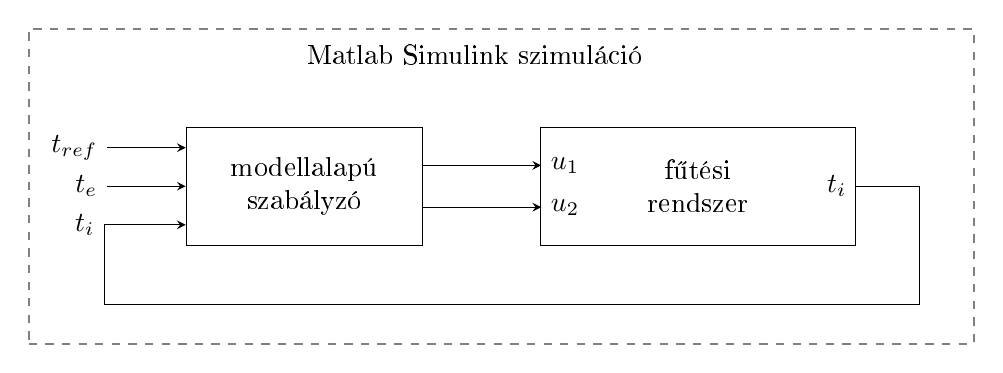
\begin{tikzpicture}[>=stealth,
	outer/.style={draw=gray,dashed,thick,inner sep=5pt}]

	% nagy blokkok
	\node[draw,rectangle, minimum height=1.5cm,minimum width=4cm] (plant) at (5,2.5) {\parbox{2cm}{\centering fűtési rendszer}};
	\node[draw,rectangle, minimum height=1.5cm,minimum width=3cm] (Control) at (0,2.5) {\parbox{2.5cm}{\centering modellalapú\\szabályzó}};
	
	% szaggatott vonal
	\node[draw,outer,rectangle, minimum height=4cm,minimum width=12cm,
	label={[label distance=-0.1cm, anchor=north]100:Matlab Simulink szimuláció}] (keret) at (2.5,2.5) {};
	
	
	% szabályzott mennyiségek
	\draw [->] (Control.10) node[right]{} -- +(15mm,0) node[right]{${u_{1}}$};
	\draw [->] (Control.350) node[right]{} -- +(15mm,0) node[right]{${u_{2}}$};
	
	%\draw[->] (Control.350) node[left]{} --  (plant.187) node[right]{${u_{2}}$};  %node[above left]{$\alpha_{radiator}$}; 
	%\draw[->] (Control.10) node[left]{} --  (plant.173) node[right]{${u_{1}}$} ;
	
	%\draw[->] (d.0) node[left]{heat [W]} ->  ++(3,0) ->  (house.180);
	
	
	% szabályzó bemenetei
	% a -| és |- máshogy fog törni, ha unconstraintelt.
	\draw [->] (plant.0)  node[left]{$t_i$} -|++(0.8,-1.5) -| ++(-9.25,0) |-  ++(-1.1,0) |- node[left]{$t_i$} (Control.198);
	
	%++(1.5cm,0) -- (2cm,0pt) -- (2.5cm,10pt);
	%\draw [->] (plant.0) node[left]{$t_i$ [\si{\celsius}]} -|++(1,0)|- -|++(-2.5,0)|- (Control.198) node[right]{}; %++(1.5cm,0) -- (2cm,0pt) -- (2.5cm,10pt);
	\draw [<-] (Control.180) node[right]{} -- +(-10mm,0) node[left]{$t_{e}$};
	\draw [<-] (Control.162) node[right]{} -- +(-10mm,0) node[left]{$t_{ref}$};
	
	%\draw[->] (House.180)  node[right]{${T_i}$} -| ++(-5.5,2)  |- (Control.180) ;
	%\draw[->] (d.20) -| ++(1,-1) |- (y.350);
	
	%\path 
	%(d.150)	 edge[<->] 	node[anchor=north,above]{valvePercent}	(y.270);
	
	\end{tikzpicture}

	\caption{A szimulációban szereplő elemek kapcsolata}
	\label{controlloop}
\end{figure}

%\begin{tikzpicture}[>=stealth,remember picture]
%\node[draw,rectangle,inner sep=0.5cm] (y) at (0,0) {$A$};
%\node[draw] (d) at (0,2) {%
%%	\begin{tikzpicture}[remember picture]
%%	\matrix [matrix of math nodes] (mat)
%%	{
%%		B & \phantom{C}   \\
%%		\phantom{B} & C \\
%%	};
%%	\end{tikzpicture}
%%};
%%\draw[->,shorten >= 6pt] (y.west) -| ++(-1,1) |- (mat-1-1);
%%\draw[->,shorten >= 6pt] (y.west) -| ++(-0.8,1) |- (mat-2-1);
%%\draw[->] ($(mat-2-2)+(14pt,0)$) -| ++(0.8,-1) |- (y.east);
%%\draw[->] ($(mat-1-2)+(14pt,0)$) -| ++(1,-1) |- (y.east);
%\end{tikzpicture}





\begin{formal}
%A munka elkezdésekor egy Simulink példa hálózatból indultam ki. Mivel a Matlab szimulációban a légbefúvásos fűtés modelljének teljesítmény kimenete van, olyan modellt szerettem volna felírni, ami beilleszthető az eredeti légbefúvó rendszer helyére. A ház hőveszteségeit a Matlab számolja\footnote{Pontosításra szorul ez a modell is, mert valószínűleg csak a konvektív hővezetéssel számol (a sugárzásival pedig nem). A légbefúvás a ház levegőjét melegíti. Ám a modellben a ház hőtároló tömege nem jelenik meg, csak egy hőellenállás a veszteségek modellezéséhez.}, ebből pedig adódik a szoba levegőjének hőmérséklete. A rendszer szabályozását így visszavezettem a leadott teljesítmény szabályzására. A levezetett egyenletnek köszönhetően egy teljesítményigényhez meg tudom majd mondani hogy mennyire kell a szabályzószelepeket kinyitni.

%Angol nyelvű szakirodalomból pl. Gouda2000 alapján számolva irreális teljesítményértékeket kaptam (150kW), tovább keresve magyar nyelvű irodalmat is áttekintettem.

%Az \textit{Épületgépészet a gyakorlatban}\footnote{Könyvtári könyv, Verlag. 5.11.6, 2. o.} c. könyvben szó esik fűtési rendszerek méretezéséről. Itt adatként szerepel egy épületre a szobák hőigénye\footnote{Pontosan nem tudom még, hogyan definiálják a hőigényt: mekkora kültéri hőmérsékletet vesznek pl. figyelembe, illetve hogy radiátor méretezésénél ezt nyilván felül kell becsülni.} és névleges hőmérséklete. Ehhez választanak megfelelő méretű radiátort, hogy azokban a kiszámolt sebességgel vizet keringetve a hőleadás elég legyen az adott helyiségbe.

%{\scriptsize(Ehhez figyelembe kell venni minden radiátorra a keringő víz hőmérsékletét is, különösen ha azok sorba vannak kötve és a hőmérsékletesések is jelentősek.)}

% Adottnak véve az előremenő és visszatérő hőmérsékletet az összes hőigényből számolható a víz kívánt áramlási sebessége. Ezután meghatározzák a radiátorok méretét, hogy azoknak a hőleadása megfeleljen az előírtaknak.

%A fenti példák segítenek a modellalkotásban is, felírható a radiátorok teljesítménye változó vízhőmérséklet és víz tömegáram esetén is. Természetesen a modell egyik bemenete, ez esetben a tömegáram a szabályzott mennyiség. Felteszem, hogy ezt folytonosan tudjuk szabályozni egy szelep segítségével (vagy ha ez nem életszerű, akkor kétállású szeleppel, de nagyobb frekvenciával, mint ahogy egy kazánt tudnánk ki/be kapcsolni).

A méretezési feladatot Csoknyai vezette le. \cite[359.~o.]{Herz} is. Ezek alapján vezettem le a leadott hő mennyiségét állandósult állapotra. Természetesen a felmelegedés és lehűlés idejét is figyelembe kell majd venni, de ezzel érthető módon a méretezésnél sem számolnak.

%További egyszerűsítésként elhanyagoltam a hőleadási tényező hőmérsékletfüggését is.
%Itt a hőveszteség adott. Esetünkben ezt a házra a Matlab számolja és jól méretezett rendszert tételezünk fel. Csupán azért kell a hőleadást jól felírni, hogy a felfutás, hőkapacitás, stb. során átadott energiát is belekalkuláljuk.
\end{formal}
%Persze ilyenkor egyedi esetekből indulok ki, de remélhetőleg ez paraméterezhetően elvezet az általános, többféle házra alkalmazható megoldáshoz.

%\subsection*{Nomenklatúra} az elejére.

\subsection{Hőleadás alapegyenletei}
A fűtőtestek hőleadása az alábbi alakban írható (\textit{Csoknyai} \cite[358.~o.]{Herz}):
%(A 86. oldalon $\Delta t_k$, a 358.-on $\Delta t_m$ jelöléssel találkozunk. A \cite[359.~o.]{Herz} ismét változik ugyanannak a jelölése. (\ref{termeszeteshk_359}) Ezutóbbi angol jelölés szimpatikusabb.)
\begin{equation} \label{eq_holeadas}
\dot Q_{le} = h_t ~ A_e ~ (t_{surf} - t_i)
\end{equation}
ahol
\begin{itemize}[itemsep=6pt,topsep=0pt,parsep=0pt,partopsep=0pt]
\item[] $\dot{Q}_{le}$ [\SI{}{\watt}] a leadott hő
\item[] $h_t$ [\si[per-mode = fraction]{\watt\per\meter\squared\per\kelvin}] a teljes hőleadási tényező %- ezt hőmérsékletfüggetlennek tekintem.
\item[] $A_e$ [\si{\metre\squared}] a radiátor felülete
\item[] $t_{surf}$ a fűtőtest felületi hőmérséklete\footnote{A felületi hőmérsékletet nem tudjuk közvetlenül mérni, ezért ki kell fejeznünk ismert jellemzőkkel.}
%\item[] $\Delta t_m$ [\SI{}{\kelvin}] a közepes hőmérsékletkülönbség:
\end{itemize}
\begin{equation} \label{eq_termeszeteshk_359}
\begin{aligned}
t_{surf} = \frac{t_w+t_r}{2} -t_{drop}
\end{aligned}
\end{equation}
ahol \si{\celsius}-ban szerepelnek:
\begin{itemize}[itemsep=6pt,topsep=0pt,parsep=0pt,partopsep=0pt]
	\item[] $t_i$ a szoba hőmérséklete
	\item[] $t_w$ a radiátorba befolyó, $t_r$ az onnan kifolyó víz hőmérséklete, ebből $\frac{t_w+t_r}{2}$ az átlagos vízhőmérséklet
	\item[] $t_{drop}$ hőmérsékletesés a közepes fűtővízhőmérséklethez képest\footnote{A hőleadás során a fűtőközeg és a fűtőtest felülete közötti konduktív hővezetés miatt hőmérsékletesés lép fel. A padlófűtésnél lesz ez különösen releváns, hiszen ott a felület hőmérséklete jóval alacsonyabb, mint a be- és kimenő vízhőmérsékletek átlaga: hiába fűtünk \SI{40}{\celsius}-os vízzel, a padló kb. \SI{25}{\celsius}-os lesz.}
\end{itemize}
%A hőátadási tényező is hőmérsékletfüggő, de ezzel egyelőre nem foglalkozom, állandónak tekintem.
%\begin{equation} \label{k_e}
%k_e = \frac{\dot{Q}}{A~ \Delta t_m}
%\end{equation}
%
%A hőteljesítmény hőmérsékletfüggő (361.~o.). Az $x^{1.33}$ az egyenletekben $x~ x^{1/3}$, ebből pedig $ x ~ \sqrt[3]{x}$ formában jelenik meg.
%
%
%Nominálisan $\Delta t_m$ = \SI{60}{\celsius}-ra adott érték a közepes hőmérsékletkülönbség függvényében változik:
%
\subsection{Hőfelvétel alapegyenletei}
A vízből felvett hő felírható:
\begin{equation} \label{eq_hofelvetel}
\dot Q_{fel} = c ~ (\xi\dot{m}) ~ \Delta t
\end{equation}
ahol
\begin{itemize}[itemsep=6pt,topsep=0pt,parsep=0pt,partopsep=0pt]
	\item[] $\dot{Q}_{fel}$ [\SI{}{\watt}] a vízből felvett hő, ami annak lehűléséből adódik
	\item[] $c$ [\si[per-mode = fraction]{\joule\per\kg\per\kelvin}] a víz fajhője
	\item[] $\xi$ a szabályzó beavatkozó jele, $ \xi \in [0,1]$ folytonosan változhat 0 és 1 között
	\item[] $\dot{m}$ [\si[per-mode = fraction]{\kg\per\second}] a víz tömegárama
	\item[] $\Delta t = t_w-t_r$ [\SI{}{\kelvin}] a víz lehűlésének mértéke
\end{itemize}

\subsection{Energiamérleg állandósult állapotban}
\textbf{Állandósult állapot} esetén a leadott hő egyenlő a felvettel, mivel akkor nem történik hőfelhalmozás, hőtárolás.
Azaz ekkor a radiátor hőkapacitását nem kell figyelembe vennem.

Beírva a (\ref{eq_holeadas})-be (\ref{eq_termeszeteshk_359})-t:
\begin{equation} \label{eq_holeadas2}
\begin{aligned}
\dot Q_{le} = h_t ~ A_e ~ \left( \frac{t_w+t_r}{2}-t_{drop} - t_i\right) = h_t ~ A_e ~ \left( \frac{t_w+(t_s-\Delta t)}{2}-t_{drop}-t_i\right)
\end{aligned}
\end{equation}

Ahol felhasználtuk azt is, hogy $t_r = t_s-\Delta t$, majd $\Delta t$ helyére beírhatjuk a (\ref{eq_hofelvetel})  átrendezett alakját:
\begin{equation} \label{eq_hofelvetel2}
~~\Delta t = \frac{\dot Q_{fel}}{c ~ \xi\dot{m}}
\end{equation}

Beírva (\ref{eq_holeadas2})-ba (\ref{eq_hofelvetel2})-t:
\begin{equation} \label{holeadas3}
\begin{aligned}
\dot Q_{le} ~=~ & h_t~ A_e\left( t_w-\frac{\dot Q_{fel}}{2~c ~ \xi\dot{m}}-t_{drop}-t_i\right)  \\[18pt]
%\Delta t_m &\triangleq  t_w-t_i-\frac{\dot Q_{fel}}{2~c ~ \dot{m}}
%\\[18pt]
\dot Q_{le} + \frac{h_t ~ A_e ~ \dot Q_{fel}}{2 ~ c ~ \xi\dot{m}} ~ = ~ & h_t ~ A_e ~\left( t_w-t_{drop}-t_i\right) \\[24pt]
2 ~ c ~ \xi\dot{m} ~ \dot Q_{le} + h_t ~ A_e ~ \dot Q_{fel} ~ = ~ &  h_t ~ A_e ~ 2~ c~ \xi\dot{m} ~\left( t_w-t_{drop}-t_i\right)
\end{aligned}
\end{equation}

\textbf{Csak abban az esetben, ha} $\dot Q_{le}=\dot Q_{fel}$:

%(meggondolandó hogy a hőkapacitások szerepe hogy alakul...)


\begin{equation} \label{eq_holeadas4}
\begin{aligned}
~~~~~~\dot Q (2 ~ c ~ \xi\dot{m} + h_t ~ A_e) & ~=~ 2 ~ h_t ~ A_e ~ c~ \xi\dot{m} ~(t_w-t_{drop}-t_i) \\[18pt]
~~~~~~\dot Q &~=~ \frac{2~c~\xi\dot{m}~h_t~A_e}{2 ~c ~ \xi\dot{m} + h_t ~ A_e}~(t_w-t_{drop}-t_i)
\end{aligned}
\end{equation}

Ez adja meg a fűtési rendszer által szolgáltatott teljesítményt állandósult állapotban.
A fenti képletben a hőleadási tényezőt hőmérsékletfüggőnek is lehet venni, \cite{CHOLEWA2013599} mérései alapján.

\textbf{Állandósult állapotra a szükséges beavatkozójel adott kimenő teljesítményhez:} \ref{eq_holeadas4} egyenletet kell $\alpha~\dot{m}$-ra (ill. csak $\alpha$-ra) rendezni.

Mivel a hőleadást, hőtárolást Simscape-ben valósítottam meg, a radiátorba bemenő hőt kell csak kiszámítani. Erre meg kell vizsgálni, hogy az állandósult állapotbeli képlet helyes-e.

\begin{formal}
	\textbf{Megjegyzés:} A radiátorba bekerülő teljesítményt a $t_w-t_r$ szabja meg (\ref{eq_hofelvetel}. egyenlet), viszont itt $t_r$-t kiejtettem az egyenletekből. Viszont a \textit{REHVA Guidebook}
	%(REHVA alacsony hom. futés és magas hom. hutés by Bjarne Olesen et. al.)
	\cite{RehvaGuidebookNo7} szerint a $\Delta t= t_w-t_r$-re szabályozással megtakarítás érhető el. Meg kell vizsgálni, reális-e mindkét paraméter mérése, radiátorok esetén, vagy csak padlófűtésnél.
\end{formal}

%\subsection{Javítás a radiátormodellen}
%
%A közepes vízhőmérséklet, a közepes felületi hőmérséklet is jöhet kimeneten ahhoz, hogy a steady-state model számolhassa a bemenő hőmérsékletet.




\section{Hőátadás tranziensének modellje}\label{section:dinamikus}







% \subsubsection*{Nomenklatúra}

A különböző hőtároló elemek feltöltődése szimulálva adja a dinamikus viselkedést.

%A modell kimenetén külön szerepelhet a sugárzás és a konvekció.

\subsection{Hőkapacitás}

Katalógusból radiátorok tömege és a bennük lévő víz térfogata leolvasható. A hőkapac számítása:

\begin{equation} \label{eq_hotartalom}
Q = c_{m} ~ m_m ~ \Delta t_k + c_{w} ~ m_w ~ \Delta t_k
\end{equation}

Ahol m a material, azaz a fűtőtest anyagára utal, w pedig a víz mennyiségére. A hőmennyiség joule-ban adott.


%\subsection{Hőleadás hőmérsékletfüggése}


\subsection{Sugárzó és konvektív teljesítmény szétválasztása}

A \textit{REHVA Guidebook} \cite{RehvaGuidebookNo7} címében is szerepel az \textit{alacsony hőmérsékletű fűtés} fogalom. Ez nem paradoxon, csupán azt jelenti, hogy a fűtőfelületek hőmérséklete az átlagosnál alacsonyabb. A levegőnél csak néhány fokkal magasabb hőmérsékletű fűtési rendszerekben pedig alacsonyabb lehet az előremenő vízhőmérséklet. Megújuló energiát használó rendszerekre ez előnyösebb, mint a régi, széntüzelésű kazánok által előállított 80--\SI{90}{\celsius}-os előremenő vízhőmérséklet.

A kis hőmérsékletkülönbség következménye, hogy a levegőnek csak kevés hőt képes leadni a rendszer. Nagyobb részt sugárzással működnek ezek a rendszerek, melyet a fűtetlen felületek nyelnek el. Ezért sugárzó (radiatív) hőátvitel esetén szokásos a $t_{AUST}$ jelölés, ami a fűtetlen felületek hőmérsékletét jeleni\footnote{AUST: Average unheated surface temperature}.

A sugárzási hőtranszfer alapegyenletét a Stefan-Boltzmann törvény adja


\begin{equation} \label{eq_stefan_boltzmann}
\begin{aligned}
\dot Q_{r} &= \sigma T_{surf}^4
\end{aligned}
\end{equation}

ahol
\begin{itemize}[itemsep=9pt,topsep=0pt,parsep=0pt,partopsep=0pt]
	\item[] $\sigma$ a Stefan-Boltzmann állandó [\si{W~m^{-2}.K^{-4}}] %\si[per-mode=fraction]{W/m^2K^4}% \si[per-mode=fraction]{\watt\per\metre\squared\per\kelvin\squared\squared} %eh [\si[per-mode = fraction]{\watt\per\metre\squared\per\kelvin^4}]
	\item[] $T_{surf}$ [\si{\kelvin}] a termodinamikai, azaz kelvinben mért felületi hőmérséklet.
\end{itemize}


(\textit{Kilkis} \cite{KILKIS1994} ):

\begin{equation} \label{eq_radiant_kilkis}
\begin{aligned}
\dot Q_{r} &= U_r ~ A~ \left(t_{surf}-t_{AUST}\right)\\[8pt]
U_r&=rF\sigma\\
r&=4 \left(\frac{T_{surf}}{2}+\frac{T_{AUST}}{2}\right)^3
\end{aligned}
\end{equation}


ahol
\begin{itemize}[itemsep=9pt,topsep=0pt,parsep=0pt,partopsep=0pt]
	\item[] $T_{surf}, T_{AUST}$ [\si{\kelvin}] a termodinamikai, azaz kelvinben mért hőmérséklet.
	\item[] $c$ [\si[per-mode = fraction]{\joule\per\kg\per\kelvin}] a víz fajhője
%	\item[] $\xi$ a szabályzó beavatkozó jele, $ \xi \in [0,1]$ folytonosan változhat 0 és 1 között
%	\item[] $\dot{m}$ [\si[per-mode = fraction]{\kg\per\second}] a víz tömegárama
%	\item[] $\Delta t = t_w-t_r$ [\SI{}{\kelvin}] a víz lehűlésének mértéke
\end{itemize}

A sugárzó hőleadási tényező bevezetésével linearizálhatjuk a hőleadást, a hőleadás így egyszerűen lineárisan függ majd a hőmérséklet-különbségtől. Gyakran összevonják a konvektív és a sugárzási hőátadási tényezőt.

\textit{Cholewa} \cite{CHOLEWA2013599} a $h_r$ paramétert méréssel határozta meg. (5) egyenlet.



\begin{equation} \label{eq_radiative_hr_linear}
\dot Q_{r} = h_r ~ A ~ \left(t_{surf}-t_{AUST}\right)
\end{equation}

ahol
\begin{itemize}[itemsep=3pt,topsep=0pt,parsep=0pt,partopsep=0pt]
	\item[] $\dot{Q}_{r}$ [\SI{}{\watt}] a leadott sugárzó hő
	\item[] $h_r$ [\si[per-mode = fraction]{\watt\per\meter\squared\per\kelvin}] sugárzó hőleadási tényező
	\item[] $A$ [\si{\metre\squared}] a padló felülete
	\item[] $t_{surf}$ [\SI{}{\kelvin}] padló hőmérséklete
	\item[] $t_{AUST}$ [\SI{}{\kelvin}] fűtetlen felületek átlagos hőmérséklete - a fal hőmérsékletének veszem a Simscapeben
\end{itemize}


%\newpage

%Fun facts:
%~
%\begin{itemize}[itemsep=6pt,topsep=0pt,parsep=0pt,partopsep=0pt]
%	\item A falakra az $\alpha$ = 10 \si[per-mode = fraction]{\watt\per\meter\squared\per\kelvin} érték a sugárzó és konvektív hőleadást is tartalmazza. A konvektív hőleadás függ a felületi áramlási sebességtől: falsaroknál ez az érték alacsonyabb, kb. a fele.
%	\item A sugárzó hő a Stefan-Boltzmann törvény alapján függ az emisszivitástól. (Annak a mértéke, hogy a test a feketetesthez képest mennyi hőt bocsát ki). A hőmennyiség a hőmérséklet negyedik hatványával arányos. A \textbf{sugárzott hő meghatározásához} még meg kell keresni és be kell írni a Simscape blokkba a megfelelő együtthatókat. Valami általános összefüggést kell találni, hogy a radiátor milyen arányban melegíti a külső falat, ahol van, ill. az ablakra milyen hatással van: még nem kezelem le ezeket az aszimmetriákat, hanem minden hőmérsékleteloszlást homogénnek veszek. A Stefan-Boltzmann törvény direkt alkalmazása helyett a szabványokban és irodalomban található közelítésekkel élek.
%	
%%	\item A $q_r$ [\si[per-mode = fraction]{\watt\per\meter\squared}] \textit{radiant heat flux density} a \cite{CHOLEWA2013599} T. Cholewa
%%	%\footnote{On the heat transfer coefficients between heated/cooled radiant floor and room. \\ DOI: http://dx.doi.org/10.1016/j.enbuild.2013.07.065}
%%	(5.) egyenlet alapján számítható de az a geometriától is nagyban függ. Helyette Kilkis1994 (4) és (6) javasolt, illetve a \cite{CHOLEWA2013599}-ból is lehet mért értékekkel számolni / a szabványok ajánlását használni.
%
%
%	\item A hőhidak a hőveszteségek meglepően nagy részéért felelősek, jelentős hibát követünk el, ha ezekkel nem számolunk. Az energetikai tanúsítvány számol ezekkel, így a modellben a veszteséghez ezt is hozzá lehet adni.
%	
%	
%	\item \cite[5.188.~o.]{watson2002radiant} szerint az operatív hőmérséklet $t_{op}~=~\frac{h_rT_{mrt}~+~h_cT_{air}}{h_{tot}}$, ahol $T_{mrt}~=~\frac{\sum\limits_{k=1}^{n}A_k\epsilon_kT_k}{\sum\limits_{k=1}^{n}A_k\epsilon_k}$. Az $\epsilon$ emittancia a StefBol képletből való.
%	
%	
%\end{itemize} 
%
%Fűtött padló, falak, mennyezet esetén jelentős szerepe van a sugárzó hőleadásnak.
%
%\begin{itemize}[itemsep=0pt,topsep=0pt,parsep=0pt,partopsep=0pt]
%	\item A.Laouadi / Building and Environment 39 (2004) 421 – 431 - p424, eq. 10-11: radiant heat transfer model - (11)-es egyenlet
%	\item TEMPERATURE CONTROL STRATEGIES FOR RADIANT FLOOR HEATING SYSTEMS, Zhi Long Zhang: 40.o.  
%%	\item \cite{CHOLEWA2013599} T. Cholewa et al. / Energy and Buildings 66 (2013) 599–606 - Table 5: coefficient
%%	\item Kilkis1994 A simplified model for radiant heating and cooling panels: itt van képlet sugárzóra
%	\item Kiegészítés: \cite[349.~o.]{Herz}
%\end{itemize}  

\section{Radiátor modellje}

A képletben élhetünk azzal a közelítéssel, hogy $\Delta t_k=\frac{t_{ws}+t_{wr}}{2}-t_i$. Ezzel a következő alakban számolhatunk:

\textit{\ref{eq_holeadas4}. egyenletben} szereplő paraméterek értéke:

\subsection{Paraméterek}
A felmelegedéskor és lehűléskor a pontos hőleadást akkor tudjuk modellezni, ha ismerjük a radiátor hőkapacitását. Ehhez tudnunk kell, hogy a radiátorban mennyi víz van, illetve hogy a radiátortest milyen nehéz.
A radiátorokat mindig az adott helyiséghez méretezik, ezért az adatokat leolvasással / katalógusból kapjuk normál esetben. A modellezéshez választanom kellett egy típust. Itt még csak paraméteresen kellene megadni az értékeket, vagy előbb a ház modelljét, hőszükségletét felírni, hiszen a házhoz tervezzük a fűtést és nem fordítva.

Radiátor katalógusokból\footnote{Purmo Ventil Compact - purmo.com/hu/termekek/lapradiatorok/purmo-ventil-compact.htm} azt találtam, hogy az egyes radiátor típusokra ezek a paraméterek milyen értékűek.

% Lapradiátor használatát feltételeztem, erről kell egy kép.

\begin{table}[H]
	\centering
	
	\renewcommand{\arraystretch}{2} % to increase cell height
	\taburulecolor{gray}
	
	%\begin{tabular}{|p{0.8cm}|p{1cm}|p{1cm}|p{1cm}|p{1cm}|p{1cm}|p{1cm}|p{1cm}|}
	
	\newcolumntype{C}[1]{>{\centering\arraybackslash}p{#1}}
	\newcolumntype{R}[1]{>{\raggedleft\arraybackslash}p{#1}}
	
	\begin{tabu}{|p{4cm}|p{3cm}|p{3cm}|p{3cm}|c|}
		\cline{2-5}
		\multicolumn{1}{l|}{} 	& Komponens & hőleadás módja & Hőtároló tömeg & Fajhő \\ \cline{2-5}
		\multicolumn{5}{c}{}\\ \hline
		% header
%		\multirow{2}{*}
%		{Radiátor} & \multicolumn{2}{c|}{Time} \\	\cline{2-3}
%		& First flight & Second flight\\ \hline
		
		
		\multirow{2}{*}
					{Radiátor} 	 & Víz 		&	&  	&	\\  \cline{2-5}
								 & Fémtest 	&	& 	& 	\\  \hline
								 
		\multicolumn{5}{c}{}\\ \hline
		
		\multirow{3}{*}
					{Padlófűtés} & Víz 		&	&  	&	\\  \cline{2-5}
								 & Födém 	&	&  	&	\\  \cline{2-5}
								 & Padló burkolat 	& 	&	& 	\\  \hline
	\end{tabu}						
		% entries - event names aligned left with multicolumn
%		\multicolumn{1}{|l|}{flightHAT turned on} 	& & \\ \hline
%%		{|p{3cm}|p{1cm}|p{3cm}|p{3cm}|p{3cm}|}
%		%{p{1.5cm}|C{0.8cm}|C{0.8cm}|C{0.8cm}|C{0.8cm}|C{0.8cm}|C{0.8cm}|C{0.8cm}|C{0.8cm}|}
%		%\multicolumn{1}{l}{}&\multicolumn{8}{l}{SDO header (első adatbyte) - master kérése}
%		%\\ 		\cline{2-9}\cline{2-9}
%		\hline
%		felület& méret & kalorikus hőátbocsátási tényező    & hőtároló tömeg & hőkapac
%		
%		\\ \hline
%		külső fal & 4.5 \si{\metre\squared} & 2 \si[per-mode=fraction]{\watt\per\metre\squared\per\kelvin} & 4.5*200kg & e.g. 4.5*200*840 \si[per-mode=fraction]{\joule\per\kelvin}
%		\\ \hline
%		ablak & 4 \si{\metre\squared} & 4 \si[per-mode=fraction]{\watt\per\metre\squared\per\kelvin} & 0 & 0
%		\\ \hline
%		belső válaszfalak & 50 \si{\metre\squared} & 7 & 50*100kg & 50*100*840	
%		\\ \hline
%		padló & 16 \si{\metre\squared} & 11 & 16*200kg & 169*200*840	
%		\\ \hline
%		mennyezet & 16 \si{\metre\squared} & ? rad / conv &  & 	
%%		\\ \hline

	
	\caption{Fűtőtestek termikus tulajdonságai}
	\label{table-sdotypes}
\end{table}


Ismert a radiátor hossza, magassága, konstrukciója. Ezalapján a
tömege, illetve az acél hőkapacitása alapján a radiátortest hőkapacitása katalógusadatként szerepel.
A szimulációban a  Simscape termikus hőtároló elem blokk a víz térfogata%, a víz fajhője még egy hőtároló elem.

\subsection{A modell validálása}

A \ref{eq_hofelvetel}. egyenlet meglehetősen általános. Ha mérjük az előre- és visszamenő víz hőmérséklet-különbségét, a tömegáram függvényében meghatározható a felvett hő.


\section{Padlófűtés modellje}

A padlófűtések felépítése az alábbi ábrán található. Egy hőszigetelő rétegre kerülnek a műanyag csövek, bizonyos elrendezésben. Erre híg betont öntenek, hogy az a csövek teljes felületét körbevegye, ne alakuljanak ki zárványok. Ha a beton nem veszi teljesen körbe a fűtéscsöveket, a padlófűtés teljesítménye lecsökken.

\begin{figure}[H]
	\centering
	% trim={<left> <lower> <right> <upper>}
	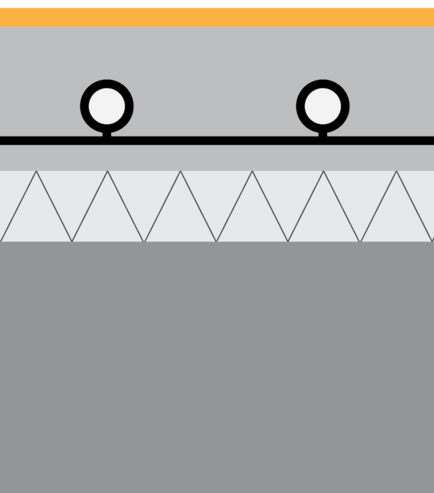
\includegraphics[trim=0 0 0 0, clip,width=0.25\textwidth]{figures/ISO11855typeA}
	\caption{Padlófűtés felépítése}
	\label{fig:futotest-padlofutes}
\end{figure}

\textit{Olesen} számításait használtam a méretezéshez.
 

Nyilvánvalóan nehéz lenne a felírt modellt egyénileg validálni, főleg hogy sehol sem találkoztam ilyen formában felírt képlettel a szakirodalomban. Szerencsére Cholewa \cite{CHOLEWA2013599} és Koca \cite{Koca} végzett méréseket falfűtés és mennyezetfűtés esetére. Ezen mérési eredmények paramétereit helyettesítettem be a hőleadás egyenletébe ahhoz hogy eldöntsem, helytálló-e a felírt modell. Az említett publikációkban minden adat rendelkezésre áll. A következő eseteket vizsgáltam:

\begin{table}[H]
	\vspace{12pt}
	\centering
	\renewcommand{\arraystretch}{1.4} % to increase cell height..
	\begin{tabular}{
			l
			S[table-format=-3.2]
			S[table-format=-3.2]
			S[table-format=-3.2]
			S[table-format=-3.2]
			S[table-format=-3.2]
			%cccc
		}
		%\hline
		\multicolumn{1}{c}{Paraméter} & \multicolumn{5}{c}{Cholewa mérései}\\%& \multicolumn{1}{c}{dummy} \\
		\hline%\cline{1-2}
		%	$T_{water}$    & Description & Price & (\$) \\
		%	\hline
		$T_{water},\si{\celsius}$      								& 30	& 30	& 40	& 50	& 55   		\\
		%$\dot{m}$ [\si[per-mode=fraction]{\kilogram\per\second}]  	& 0.0167& 0.055	& 0.0167& 0.0167& 0.055    	\\
		$\dot{m}$ [\si[per-mode=fraction]{\kilogram\per\minute}]  	& 1		& 3		& 1		& 1		& 3		    \\
		$T_{surf}$													& 25.3	& 26.2	& 32    & 37.4  & 42.4		\\
		$T_{a0.6}$       											& 22.3  & 23.3 	& 26.9	& 30.8  & 34.3 		\\
		$h_{total0.6}$ \small{$\left[ \frac{\si{\watt}}{\si{\metre\squared\kelvin}} \right]$ }
		& 8.7   & 9.4  	& 9.7  	& 10.5  & 10.8  	\\[5pt] \hline 
		%$\Delta T$       											& 3     & 2.9	& 5.1  	& 6.6   & 8.1 		\\[5pt] \hline 
		$q_{total}$ \small{$\left[ \frac{\si{\watt}}{\si{\metre\squared}} \right]$}
		& 25.1  & 26.4  & 47.8  &  68.8	& 88.4   	\\[5pt] 		
		$q_{formula}$ \small{$\left[ \frac{\si{\watt}}{\si{\metre\squared}} \right]$}
		& 24.6  & 26.7  & 46.3  &  64.5 & 85.5   	\\%[5pt] \hline 
		%Pontosság \%												& 98	& 101	&  97	& 93.75 & 96.7		\\
		\hline
	\end{tabular}
	\caption{A \ref{eq_holeadas4}. képlettel kapott eredmények és a \cite{CHOLEWA2013599} és \cite{Koca} eredményeinek összevetése}
	
\end{table}


% Az 1.1 méréseket használva rendre 10%-kal alábecsültük a hőt.
{\Large }


A hőleadás egyenletével számolt és a fent hivatkozott, méréssel kapott eredmények elég jól követik egymást. Padlófűtésnél a padló felületi hőmérséklettel számoltam, ugyanis a padló hőmérséklete jóval alacsonyabb, mint a fűtővíz hőmérséklete.
A fenti publikációkban figyelembe vették a hőleadási tényező hőmérsékletfüggését.\footnote{Intuitívan is belátható, hogy melegebb testnek nagyobb a konvektív hőleadási tényezője. A konvektív hőátadás mértéke nagyban függ attól, hogy a felületen milyen sebességgel áramlik a levegő, hiszen a forró tea gyorsabban hűl, ha fújjuk, illetve szélben a kinti hőmérséklet kisebbnek érződik. Hasonlóan melegebb tárgy esetén a légáramlás felgyorsul, amiatt hogy a melegebb levegő felfelé száll.} %Nagyobb felületi légáramlás tehát megnövekedett konvektív hőátadást eredményez.}
Azaz a felfutási tranziens során is változik a hőátadási tényező.



\pagebreak
\section{Modellek tesztje}

\subsection{Radiátor unit test}

\subsubsection{Állandósult állapot numerikus modellje}

Annak ellenőrzése, hogy a \ref{holeadas4} egyenlet jó-e. Azaz elfogadható-e ez a közelítés állandósult állapotban, illetve a tranziens alatt mennyire feasible. 

Az egyenletben a mintavételi idő egy szorzóként jelenik meg, 

Az egyenlet wattban adja a kimenetét.
A teszt egy formája lehet, ha a gyári adatokat (fűtési teljesítmény) összevetem az általam számoltakkal.

\subsubsection{Tranziens Simscape modellje}
A bejövő hő függvényében a hőleadás tranziensei. A bejövő hőt a képlet numerikusan számítja. A tranzienst viszont Simscape-ben szimulálom. Ez folytonos rendszert feltételez.

\subsubsection{Szabályzás célja}

Állandósult állapotban olyan bemenő hőáramot elérni, ami épp fedezi a veszteségeket.

\subsection{Padlófűtés unit test}

\chapter{Identifikáció}\label{chap:ident}


A szabályzó tervezésénél használt szakaszmodell a Simulinkben megvalósított fizikai modell viselkedését leíró lineáris rendszer. Ebben a fejezetben a korábbiakban ismertetett hálózatot identifikálom.
\begin{figure}[h]
	\centering
	\begin{figure}[h]
	\centering
	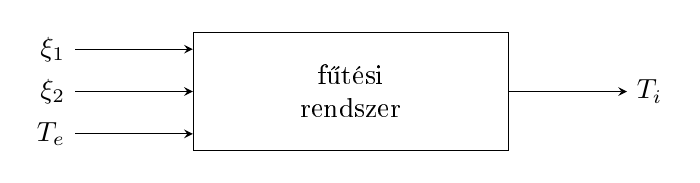
\begin{tikzpicture}[>=stealth,
	outer/.style={draw=gray,dashed,thick,inner sep=5pt}]
	
	% nagy blokkok
	\node[draw,rectangle, minimum height=1.5cm,minimum width=4cm] (plant) at (0,2.5) {\parbox{2cm}{\centering fűtési rendszer}};
	%\node[draw,rectangle, minimum height=1.5cm,minimum width=3cm] (Control) at (0,2.5) {\parbox{2.5cm}{\centering modellalapú\\szabályzó}};
	
	% szaggatott vonal
	%\node[draw,outer,rectangle, minimum height=4cm,minimum width=12cm,
	%label={[label distance=-0.1cm, anchor=north]100:Matlab Simulink szimuláció}] (keret) at (2.5,2.5) {};
	
	
	% plant bemenetei
	\draw [<-] (plant.165) node[left]{} -- +(-15mm,0) node[left]{${\xi_{1}}$};
	\draw [<-] (plant.180) node[left]{} -- +(-15mm,0) node[left]{${\xi_{2}}$};
	\draw [<-] (plant.195) node[left]{} -- +(-15mm,0) node[left]{$T_{e}$};
	\draw [->] (plant.0) node[left]{} -- +(15mm,0) node[right]{$T_{i}$};
	
	% szabályzó bemenetei
	% a -| és |- máshogy fog törni, ha unconstraintelt.
	%\draw [->] (plant.0)  node[left]{$t_i$} -|++(0.8,-1.5) -| ++(-9.25,0) |-  ++(-1.1,0) |- node[left]{$t_i$} (Control.198);
	
	%\draw [<-] (Control.180) node[right]{} -- +(-10mm,0) node[left]{$t_{e}$};
	%\draw [<-] (Control.162) node[right]{} -- +(-10mm,0) node[left]{$t_{ref}$};
	\end{tikzpicture}
	\caption{A szimuláció felépítése}
	\label{tikz:simulation}
\end{figure}

	\caption{A szabályzott szakasz összevont modellje}
	\label{tikz:simulation}
\end{figure}

A Simulinkben vizsgálójeleket használok: a több bemenetű, egy kimenetű rendszert egyszerre csak egy bemenetén gerjesztem. A tömegáramot szabályzó szelepek nyitott és csukott állapot között folytonosan állíthatók, 0 és 1 közötti beavatkozó jellel. A külső hőmérsékletet a modell kelvinben kapja, kimenete a belső hőmérséklet.

A szelepekkel való beavatkozás hiányában a $T_i$ belső és $T_e$ külső hőmérséklet különbsége (a helyiség időállandójának megfelelően) kiegyenlítődik.

 %(\textit{\ref{fig:valve-step}. ábra}). 
% a kimeneti változást létrehozó hatás egyértelműen beazonosítható kell hogy legyen.

\section{A szakasz ugrásválasza}

Lineáris hálózatoknál gyakori vizsgálójel az egységugrás, illetve az impulzusgerjesztés. Az identifikációhoz ugrásválaszt vizsgáltam, de mivel a rendszernek 3 bemenete van, ezekre nem egyszerre, hanem időben eltolva adtam ugrásgerjesztést, mindig megvárva, hogy az előző hatás tranziense lecsengjen. A következőkben viszont nem csak a tranziensek a fontosak, hanem a végértékek is. A következő három ábrán összevethetők a szakasz tulajdonságai egyes gerjesztésekre.

\begin{figure}[H]
	\centering
	% trim={<left> <lower> <right> <upper>}
	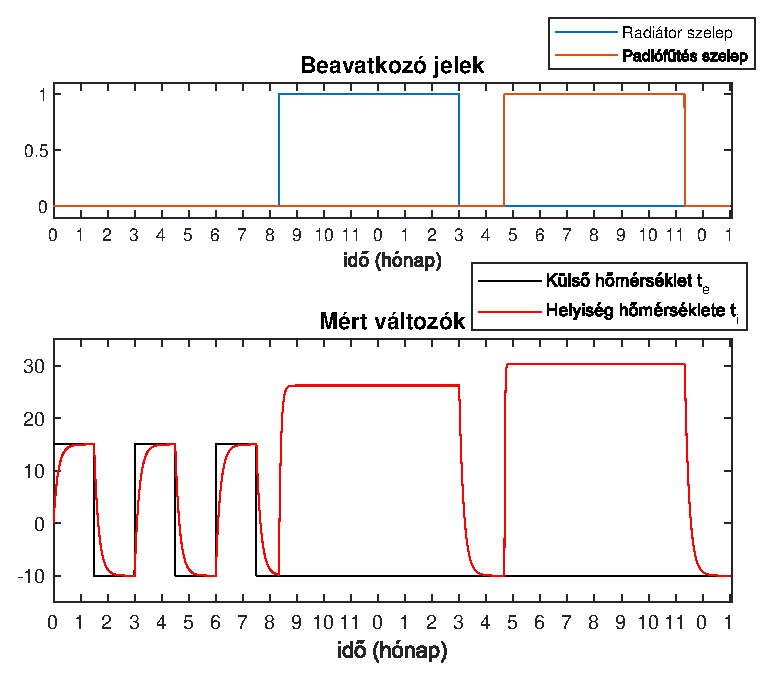
\includegraphics[trim=0 0 0 0, clip,width=0.73\textwidth]{figures/valve-step}
	\caption{Szimuláció a bemeneteket külön-külön gerjesztve}
	\label{fig:valve-step}
\end{figure}
Lineáris hálózat esetén a kimeneten a válasz az ugrásgerjesztések szuperpozícióval adódik. A fenti ábrán látható, hogy a szelepek teljes kinyitásával kb. \SI{35}{\celsius}-kal emelkedett a belső hőmérséklet. Lineáris hálózat esetén feleakkora beavatkozó jellel \SI{17.5}{\celsius}-os hőmérséklet-emelkedésre számíthatnánk.
%Ez azt jelentené, hogy ha egy szelepet kétszer jobban kinyitok, az kétszer jobban emeli meg a helyiség belső hőmérsékletét. Illetve ha a két szelepet egyszerre nyitom ki, akkor 
\begin{figure}[H]
	\centering
	% trim={<left> <lower> <right> <upper>}
	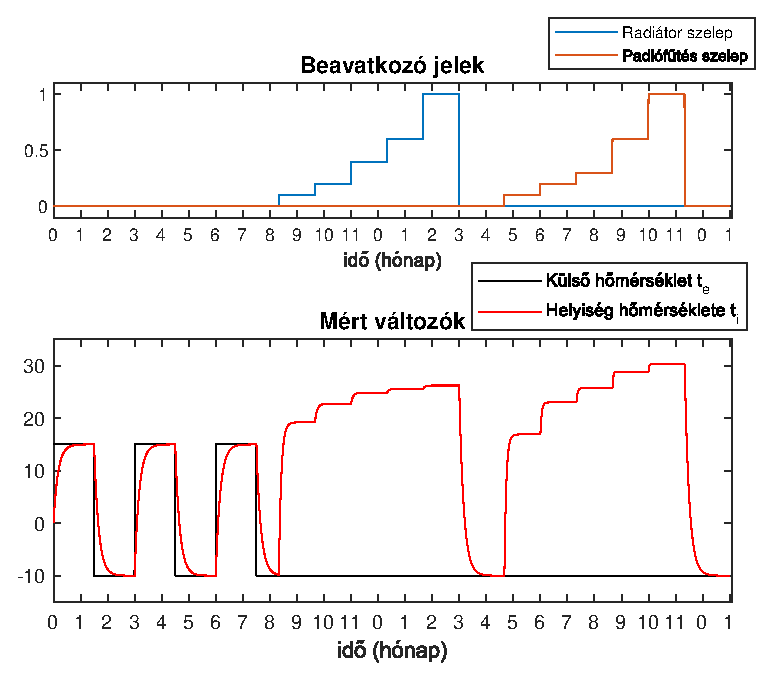
\includegraphics[trim=0 0 0 0, clip,width=0.73\textwidth]{figures/valve-stair}
	\caption{Szimuláció a szelepeket lépcsős függvénnyel gerjesztve}
	\label{fig:valve-stair}
\end{figure}

A fűtőtestekben a víz tömegáramát szelepekkel szabályozzuk. Az \textit{\ref{eq_holeadas4}. egyenlet} adja fűtőtestek által leadott hőmennyiséget, ám ez nem lineáris függvénye a tömegáramnak. A \textit{\ref{fig:valve-stair}. ábrán} látszik, hogy kétszer jobban kinyitott szeleppel $t_i$ belső hőmérséklet végértéke csak kicsivel lesz magasabb. A szelepek tehát nemlineáris bemenetek, a szuperpozíció elve nem működik\footnote{A szakasz másik nemlinearitása a szaturáció: a szelepet csak [0..1] tartományban lehet működtetni -- a szabályzótervezésnél ezt figyelembe fogom venni.}.

A $t_i$ belső hőmérséklet végértéke a tömegáramon kívül a $t_e$ külső hőmérséklettől is függ: ugyanakkora belső hőmérsékletet csak nagyobb tömegárammal, vagy nagyobb $t_w$ előremenő vízhőmérséklettel lehet tartani\footnote{Bár a vízhőmérsékletet nem szabályozom, egyes kazánok rendelkeznek külső hőmérővel, így a vízhőmérsékletet megemelve a hidegben a $t_i$ végértéke "automatikusan" azonos maradhat.}. 

\begin{figure}[H]
	\centering
	% trim={<left> <lower> <right> <upper>}
	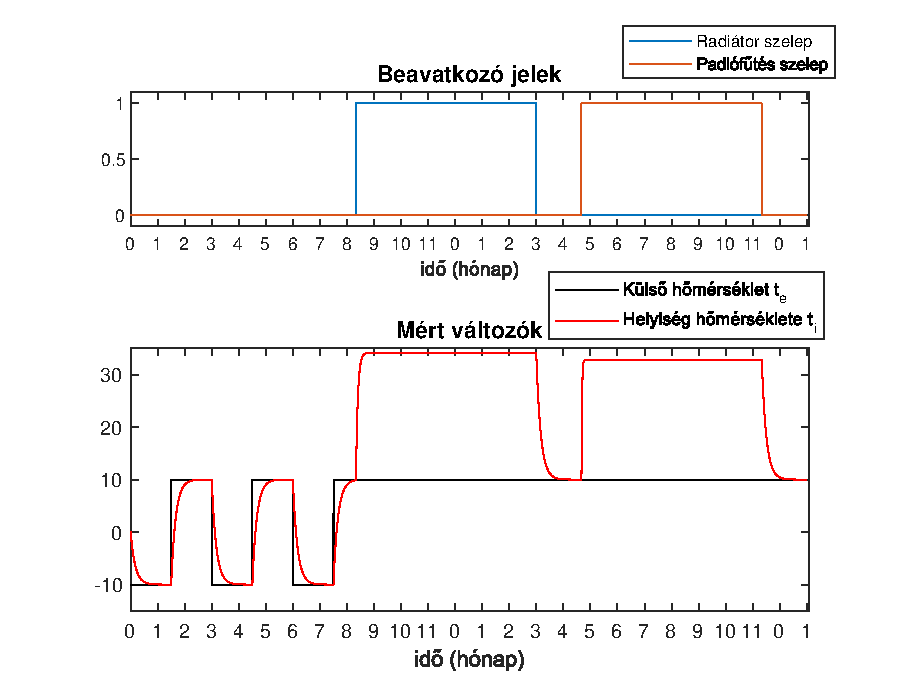
\includegraphics[trim=0 0 0 0, clip,width=0.72\textwidth]{figures/valve-step-hot}
	\caption{Szimulációs eredmények a bemeneteket külön-külön gerjesztve}
	\label{fig:valve-step-hot}
\end{figure}

Látható, hogy a különböző bemenetekre adott gerjesztések hatása a kimeneten sem számítható szuperpozícióval: \SI{20}{\celsius}-kal megemelt $t_e$ külső hőmérséklet esetén a fűtőtestek nem fognak \SI{20}{\celsius}-kal magasabb belső hőmérsékletre fűteni. Ez vonatkozik két szelep együttes kinyitására is: a hőmérséklet nem fog jelentősen megemelkedni.

A fenti hatásokat nemlineáris modellekkel lehetne lekövetni, viszont az ezekkel kapcsolatos (hiányos) ismereteim miatt erre szabályzótervezéssel nem próbálkoztam. Viszont egy nemlineáris modellt tudtam identifikálni a mérési adatokra, ami a fenti problémák egy részét kiküszöbölte.

%A Simulink modellt bemenetein gerjesztem (külső hőmérséklet \SI{40}{\celsius}, majd fűtés \SI{60}{\celsius} előremenő hőmérsékleten valve = 1 állásban.\footnote{A stratégia lehet $t_s$ előremenő hőmérséklet vagy $\xi \cdot \dot m$ tömegáram szabályzása $\alpha$ = [0..1] beavatkozójellel. })

\section{Átviteli függvény illesztése az adatokra}

Az identifikációhoz adatfájlt hozok létre, a Simulinkben IDDATA blokk a be- és kimenetek értékét mintavételi időnként rögzíti és a \textit{Base Workspace}-be (a közös változók közé) menti. Innen a \textit{System Identification} alkalmazásba betölthetőek az adatok. %A mintavételi idő először egy másodperc volt. %A Matlab Workspace-ben megjelenik egy iddata, ezt tudom az ident toolboxba importálni.
Az adatsorra átviteli függvényeket illesztek: a pólusok, zérusok a száma a Simscape modell alapján meghatározható, RC-hálózatok analógiájával. Ekkor például a radiátorok felmelegedési idejét is leköveti a modell. A teljes helyiség időállandójához képest viszont például a radiátor felmelegedése elhanyagolható. Fél órás mintavételi idő esetén a fűtőtestek egytárolós taggal helyettesíthetők. 




Célszerű az identifikációnál minél nagyobb változásokat mérni - így a rendszer teljes dinamikáját, hőtároló képességét mértem. A beállási idők körülbelül 30 naposak voltak és több periódusnyi mérésre volt szükség. 


%Nem tartottam "értelmét" 1\si{\celsius}-os step jelre identifikálni. Így beállítottam nulla kezdeti értéket a ház összes paraméterére. (Falak, fűtési rendszer, stb. Nyilvánvaló, hogy ilyenkor nem a realizmus a cél, hiszen a nagy változásokra jön elő a rendszer dinamikája.) Nulla kezdeti értékből a környezeti hőmérsékletet 0-ról 40\si{\celsius}-ra emeltem, ennek a beállási ideje több nap volt, majd visszaállítva 0\si{\celsius}-ra megvártam a lecsengést, ezután pedig a beavatkozó szelepeket teljesen kinyitottam. 

%Egy ilyen szimuláció a fenti szekvenciával kb. 50 napnyi viselkedést fog át, ez másodperces mintavételi idővel rengeteg adat, amivel meggyűlik az Ident Toolbox baja is.

%5 perces mintavételi időkkel már sokkal gyorsabban lefut a Simulinkben a szimuláció és a toolboxban az identifikáció, lénygében azonos eredményt adva.

%Viszont a mintavételi idők megváltoztatásánál, nem volt egyértelmű, hogyan reagál a Simscape vagy az MPC. A Simscape-nél kiderült, hogy a mintavételi időt manuálisan nem lehet megadni.


\begin{figure}[H]
	\centering
	% trim={<left> <lower> <right> <upper>}
	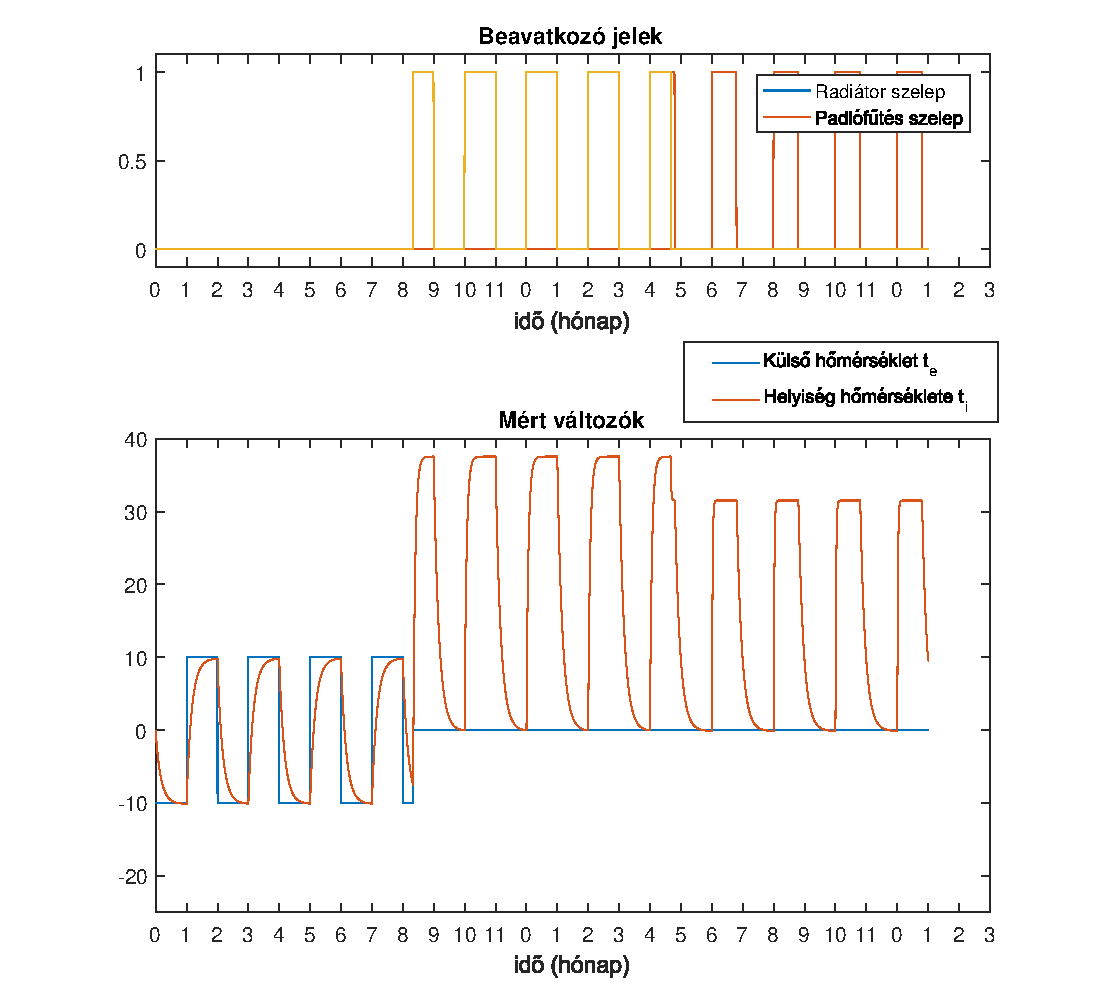
\includegraphics[trim=0 0 0 0, clip,width=\textwidth]{figures/ident-valve3}
	\caption{Identifikáció során }
	\label{fig:ident}
\end{figure}

Az identifikáció pontosságának javításához mindhárom bemeneti változó hatását több periódusra rögzítettem, 750 napnyi szimulációval. Ez fél órás mintavételi idő mellett szimulációban kevesebb, mint 1 perc alatt futott le. Az identifikációhoz a hőmérsékletet kelvinben rögzítem, mivel \si{\celsius} használata esetén az összefüggések nem lineárisak. (A kelvinben mért hőmérsékletet nevezik termodinamikai hőmérsékletnek.) A fenti esetben a beállási idők nagyjából 30 naposak az egész rendszert tekintve, ami 10 nap körüli időállandót jelent. Szakirodalom szerint a falszerkezetek időállandója megközelítőleg 5 nap, a helyiségre így reálisnak tűnik a közelítés.

Átviteli függvény identifikációjához a fenti nemlinearitásokat okozó gerjesztéseket nem vettem figyelembe. Így az átviteli függvény a rendszer jellegét követte, és a \textit{\ref{fig:valve-step-hot}. ábrán} látható külső hőmérsékletre és teljesen kinyitott szelepekre a végértékek pontosan illeszkednek.


\begin{figure}[H]
	\centering
	% trim={<left> <lower> <right> <upper>}
	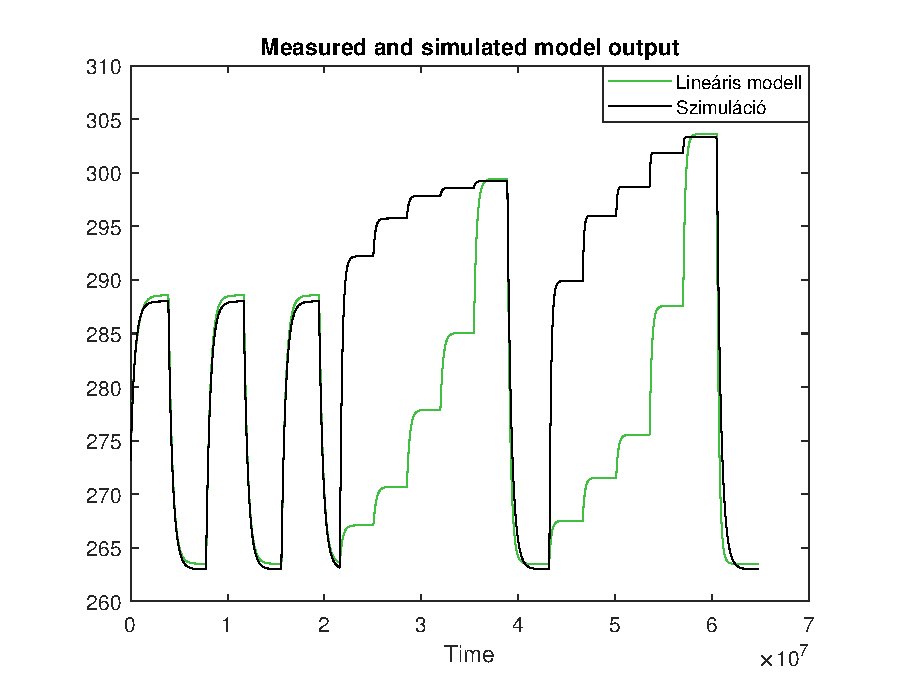
\includegraphics[trim=0 0 0 0, clip,width=0.9\textwidth]{figures/identModelOutputMatch}
	\caption{Identifikált modell pontatlansága}
	\label{fig:ident-model-mismatch}
\end{figure}

%Zérusok hatása röviden. Mit tud. Hánytárolós rendszer. Néhány kép.
%MISO identifikáció. 
%
%
%\section{Hagyományos szabályzás performanciája}
%
%PI, miért nem jó
%Csak SISO-ra működik és itt esetünkben itt több bemenetről van szó mindenképpen. Irodalom: S. Prívara et al. 
%


\pagebreak
\chapter{Szabályzó kiválasztása és analízise}\label{chap:control}

A fejezetben a Simulinkben átviteli függvényre megtervezem a szabályzást. A szabályzó választásakor világossá vált, hogy egy egyszerű PID típusú szabályzás nem képes a rendszert jól kezelni. Igaz, hogy a PID közismert és az iparban egyszerűsége miatt széles körben használt, de épületgépészeti alkalmazásnál nem olyan egyértelmű egy szabályzás performanciája. A referenciakövetést például elég egy hibahatáron belül megvalósítani, itt lazábbak a követelmények.
%A költségek és a károsanyag-kibocsátás egyre fontosabb szempont: előnyösebb, olcsóbb beavatkozó 


Már a modell identifikációját is bonyolította az egynél több bemenet. Illetve kettő van kimenetből is. A szabályzásnál különösen nehéz több bemenetű rendszerre tervezni, esetleg a modellek szétválasztásával lehetséges: külön beavatkozójel a 


Az identifikált modellekre többféle szabályzót tervezek, illetve próbálok ki.

A hasonló feladatokra leggyakrabban modell-prediktív (MPC) szabályzást használnak \cite{AFRAM2014343}. Ehhez szükség van a szakasz modelljére, ami alapján a szabályzó szimulálhatja a szakasz kimenetét. A szimuláció több mintavételi perióduson, egy predikciós horizonton keresztül fut le, minden lehetséges  beavatkozójel-sorozatra a kimenetet szimulálva.
%A csúszóablak miatt receding horizon control
Ezen sorozatok közül a legjobbat kiválasztja és egy lépést végrehajt. Ezután a szimuláció újrakezdődik. Az optimális beavatkozójelet egy költségfüggvény minimalizálásával kapja. A költségfüggvényben különböző eltéréseknek vagy abszolútértékeknek különböző súlya lehet.

Egy irodában, vagy lakásban 0.1\si{\celsius}-os vagy 1\si{\celsius}-os pontosságú hőmérsékletszabályzás közötti különbség komfortban aligha érezhető. Ám a követelmények megengedhető mértékű lazítása az energiafogyasztást nagyban lecsökkentheti.

\begin{formal}
	Ha az mpc blokknak van külső ktsg fv. bemenete, használjuk azt. Ebből kössük rá a numerikus képleteket. A teljesítmény integrálját és pillanatértékét, ill. túl gyors változását is lehet büntetni és energetikai szempontotkat (kazán hatásfoka, energia ára, napelemmel megtermelt mennyiség, azaz törés az energiaköltségben, ha egy külön blokkban megadjuk ezeket.)
\end{formal}

\section{Ismerkedés az MPC szabályzással}

\subsection*{Nomenklatúra}

\begin{itemize}[noitemsep,topsep=-8pt,parsep=0pt,partopsep=0pt,leftmargin=42pt]
	\item[\textbf{MPC}] Model Predicive Control
\end{itemize}

\vspace{12pt}


\begin{table*}[h]
	\caption{Az MPC be-és kimenetei a szabályzási körben}
	\label{nomencl_mpcsignals}
	\begin{itemize}[noitemsep,topsep=0pt,parsep=2pt,partopsep=4pt,leftmargin=42pt]
		\item[\textbf{MO}] Measured output of the plant - a visszacsatolt jel
		\item[\textbf{REF}] A referenciajel % konstans vagy tomb?
		\item[\textbf{MD}] Measured disturbance on plant input (?) - ha a zavarjelet lehet mérni, de beavatkozni azon a bemeneten nem lehet
		\item[\textbf{MV}] Manipulated variable of the plant - beavatkozó jel 
	\end{itemize}
\end{table*}
Egyéb MPC paraméterek: mintavételi idő, predikciós horizont, control horizont, súlyozás, soft vagy hard constraintek, cost, optimum (szuboptimum) , stabliltás / garanciák

%terminal constraint, online optimization, adaptive parameters

%\vspace{12pt}


\begin{figure}[h]
	\centering
	\begin{tikzpicture}[>=stealth]

			%	\node [draw,label={[label distance=1cm]90:label}] at (9,0) {Node};
			%	
			%	\node (n) at (-5,5) {n};
			%	\draw [<-] (n.north) -- +(0,5mm) node[above]{Mért értékek};
			%	\draw [<-] (n.west) -- +(-5mm,0);
			%	\draw [<-] (n.south) -- +(0,-5mm);
	
	% Szabályzási kör elemei

	% Controller
	% ----------
	\node[draw,rectangle, minimum height=3cm,minimum width=6cm,
		  %label={[xshift=1.0cm, yshift=0.3cm]Label},
		  %label={[xshift=-4.1cm, yshift=-0.7cm]Label},
		  ]
		  (MPC) at (2.3,2.5) {\parbox{2cm}{\centering MPC}};	
	
	% az MPC doboz bemenetei
	\draw [<-] (MPC.160) node[right]{MO} -- +(-15mm,0) node[left]{$T_i$};
	\draw [<-] (MPC.170) node[right]{REF} -- +(-15mm,0) node[left]{$T_{ref}$};
	\draw [->] (MPC.0) node[left]{MV} -- +(15mm,0) node[right]{$\alpha$ [\si{\percent}]};
	\draw [<-] (MPC.180) node[right]{MD} -- +(-15mm,0) node[left]{$T_e$};
	
%	\draw [<-] (MPC.160) node[right]{MO} -- +(-15mm,0) node[left]{Mért értékek};
%	\draw [<-] (MPC.170) node[right]{REF} -- +(-15mm,0) node[left]{Referenciajel};
%	\draw [->] (MPC.0) node[left]{MV} -- +(15mm,0) node[right]{Beavatkozó jel};
%	\draw [<-] (MPC.180) node[right]{MD} -- +(-15mm,0) node[left]{Mért zavarjelek};

	
	%	\node[rectangle, minimum height=1cm,minimum width=1cm] (ghostRef) at (-3,3.6) {};	
%	\node[rectangle, minimum height=1cm,minimum width=1cm] (ghostMeas) at (-3,2.85) {};	
%	\node[rectangle, minimum height=1cm,minimum width=1cm] (ghostDist) at (-3,2.15) {};
	
	%\node[draw,rectangle, minimum height=2cm,minimum width=5.5cm] (Simsc) at (9,2.5) {\parbox{2cm}{\centering fűtési rendszer Simscape}};
	%\node[draw,rectangle, minimum height=1.5cm,minimum width=3cm] (house) at (5,0) {\parbox{2cm}{\centering ház Simscape}};
	%\node[draw,rectangle, minimum height=1.5cm,minimum width=3cm] (ctr) at (0,0) {controller};
	
	
	%\draw[->] (ghostRef.0) node[left]{Referenciajel} --  (MPC.160) node[right]{REF};  %node[above left]{$\alpha_{radiator}$}; 
	%\draw[->] (ghostMeas.0) node[left]{Mért értékek} --  (MPC.173) node[right]{MO};  %node[above left]{$\alpha_{radiator}$}; 
	%\draw[->] (ghostDist.0) node[left]{Mért zavarás} --  (MPC.186) node[right]{MD};  %node[above left]{$\alpha_{radiator}$}; 
	
	%\draw[->] (ctr.191) node[right]{${u_{2}}$} -| ++(-1.7,1.3)|-  (Numeric.182) node[right]{$\alpha_{floor}$};  %node[above left]{$\alpha_{radiator}$}; 
	%\draw[->] (ctr.169) node[right]{${u_{1}}$}-| ++(-1,0.8)  |-  (Numeric.195) node[right]{$\alpha_{radiator}$} ;
	
	%\draw[->] (d.0) node[left]{heat [W]} ->  ++(3,0) ->  (house.180);
	%\draw [->] (MPC.0) node[left]{$Q_r, Q_c$ [W]} -| ++(2,-2.5)  |- (house.0) node[left]{${Q_{be}}$}; %++(1.5cm,0) -- (2cm,0pt) -- (2.5cm,10pt);
	
	%\draw[->] (house.180)  node[right]{${T_i}$} -- (ctr.0) ;
	%\draw[->] (d.20) -| ++(1,-1) |- (y.350);
	
	%\path 
	%(d.150)	 edge[<->] 	node[anchor=north,above]{valvePercent}	(y.270);
	
	\end{tikzpicture}

	\caption{Az MPC be- és kimenetei}
	\label{fig_mpcinout}
\end{figure}

%\begin{tikzpicture}[>=stealth,remember picture]
%\node[draw,rectangle,inner sep=0.5cm] (y) at (0,0) {$A$};
%\node[draw] (d) at (0,2) {%
%%	\begin{tikzpicture}[remember picture]
%%	\matrix [matrix of math nodes] (mat)
%%	{
%%		B & \phantom{C}   \\
%%		\phantom{B} & C \\
%%	};
%%	\end{tikzpicture}
%%};
%%\draw[->,shorten >= 6pt] (y.west) -| ++(-1,1) |- (mat-1-1);
%%\draw[->,shorten >= 6pt] (y.west) -| ++(-0.8,1) |- (mat-2-1);
%%\draw[->] ($(mat-2-2)+(14pt,0)$) -| ++(0.8,-1) |- (y.east);
%%\draw[->] ($(mat-1-2)+(14pt,0)$) -| ++(1,-1) |- (y.east);
%\end{tikzpicture}



\subsection{Elvárások a szabályzás teljesítményével szemben}

Az MPC hangolása során % működését, tulajdonságait meg tudjam figyelni,
lépésről lépésre fogom módosítani az alapértelmezett paramétereket, azok hatását megfigyelem.
Az MPC szintézis folyamata:% be kellene tabolni


\begin{enumerate}[noitemsep,topsep=0pt,parsep=2pt,partopsep=4pt,leftmargin=30pt]
	\item a szakaszt identifikálni kell, az átviteli függvény be- és kimeneteinek típusát be kell állítani,
	\item létre kell hozni az MPC-t a megfelelő mintavételi frekvenciával,
	\item be kell állítani a jelek fizikai korlátait és súlyukat a szabályzás költségfüggvényében,
	%\item Be kell állítani a jelek fizikai korlátait
	\item hozzá kell adni a Simulink modell Model workspace-éhez a szabályzót és megadni a nevét az Explicit MPC blokkjában (az itt található Review funciót is érdemes használni),
	\item be kell kötni a jeleket és le kell futtatni a szimulációt.
	
\end{enumerate}

%Identifikálni kell a szakaszt.

A \verb|"setmpcsignals()"| függvény használatával egy új átviteli függvényt hozunk létre, amit az MPC függvénynek odaadhatunk. Ez annyival több az identifikált tf-nél, hogy benne vannak a be-és kimenetek típusai is, aszerint, hogy az említett jelek milyen típusúak. A szakasz átviteli függvényének be- és kimeneteit meg kell nevezni, a típusokat a \ref{nomencl_mpcsignals} listából választhatjuk ki. Ezután az \verb|"mpc(tf, Ts)"| függvénnyel létrehozhatjuk az MPC szabályzót a megadott szakaszmodellre.

Ezzel még nem kaptunk használható szabályzót, mert az alapértelmezett súlyok és a normalizálatlan bemenetek miatt a legkisebb költségű beavatkozás az, ha egyszerűen nem csinálunk semmit.

A költségfüggvény akkor működik jól, ha a modellbemeneteket 1-re normáljuk. Be kell állítani tehát az MPC mért változó tulajdonságánál a modell kimenetének 1-re skálázását. 

Alapértelmezés szerint a költségfüggvény súlyai az alábbiak. A zárt szabályzási körben ezek a súlyok a hibajelet büntették a legjobban, ezért nagyon jó referenciakövetést sikerült elérni.


Követelmények a referenciajelekre:

Thermal comfort - Olesen, ISO EN 7730

Floor temperature - herz-ől is



%Az MPC szabályzót létrehoztam a toolbox-szal, az identfikált szakaszból. Beállítottam a be-és kimenetek jellegét, korlátait. A ki-és bemeneteket helyesen bekötve már működött is a szabályzás.
%Fontos, hogy helyesen válasszuk meg a mintavételi időt, illetve a súlyokat

%A kezdeti cél egy "sima" szabályzás. Kérdés, hogy egyáltalán tud-e ilyet az MPC. Gyanítom, hogy a hibaminimalizáló függvény megfelelő megadásával tud: ha egy négyzetes hibaminimalizáló van rajta, \textit{biztosan "jó"} lesz.\footnote{Bármit is jelentsen a \textit{jó} szabályzás.}



\subsection{A MATLAB MPC Toolbox elemei}
Az MPC blokknak van egy alapértelmezett költségfüggvénye, és ennek a súlyozását lehet beállítani.
Külön beállítható a szabályzási és a szimulációs horizont.
Ezek optimális beállításai 

A kezdeti MPC szabályzót egyszerűen létre lehet hozni az identifikált modellből és a bemenetek típusának megadásával. (A szelep a beavatkozó jel, illetve a plantnek van még egy bemenete, egy mérhető zavarás.) Ezután a bemenetek értékkészletét adtam meg, illetve van egy normalizáló faktor, ami a jellemző\textit{full scale}.

Az optimalizálás egy költségfüggvény minimalizálását jelenti, amiben \textit{büntetjük} a referenciajeltől való eltérést és a beavatkozó jelek \textbf{értékét vagy változását}.

A fenti a klasszikus MPC, tov. info. Baochang DING, Modern MPC című könyvében olvasható.


%\begin{lstlisting}[
%style=Matlab-editor,
%basicstyle=\mlttfamily,
%escapechar=`,
%]
%tf_19_toMPC=setmpcsignals(tf19, 'Manipulated',[2 3],'MeasuredDisturbances' ,1)
%
%tf_19_toMPC =
%
%From input "u1" to output "y1":
%   3.776e-05 s^2 + 5.958e-09 s + 8.529e-15
%--------------------------------------------
%s^3 + 0.002341 s^2 + 9.301e-09 s + 8.241e-15
%
%
%From input "u2" to output "y1":
%                 7.74 s + 0.000236
%---------------------------------------------------
%s^4 + 1.269e04 s^3 + 4262 s^2 + 3.299 s + 8.454e-06
%
%
%From input "u3" to output "y1":
%  6.361e-05
%-------------
%s + 2.637e-06
%
%Input groups:
%       Name                 Channels
%   Manipulated                 2,3
%     Measured                   1
%
%Output groups:
%       Name                 Channels
%     Measured                   1
%
%Name: tf19
%Continuous-time identified transfer function.
%Parameterization:
%    Number of poles: [3 4 1] Number of zeros: [2 1 0]
%    Number of free coefficients: 14
%    Use "tfdata", "getpvec", "getcov" for parameters and their uncertainties.
%
%Status:
%Estimated using TFEST on time domain data "tf_3in1out__68d".
%Fit to estimation data: 82.28% (stability enforced)
%FPE: 1.707, MSE: 1.706 
%
%
%>> mpc_control_slab=mpc(tf_19_toMPC,1)
%-->Converting linear model from System Identification Toolbox to statespace.
%-->The "PredictionHorizon" property of "mpc" object is empty. Trying
%PredictionHorizon = 10.
%-->The "ControlHorizon" property of the "mpc" object is empty. Assuming 2.
%-->The "Weights.ManipulatedVariables" property of "mpc" object is empty.
%Assuming default 0.00000.
%-->The "Weights.ManipulatedVariablesRate" property of "mpc" object is
%empty. Assuming default 0.10000.
%-->The "Weights.OutputVariables" property of "mpc" object is empty.
%Assuming default 1.00000.
%MPC object (created on 30-Oct-2018 20:51:50):
%---------------------------------------------
%Sampling time: 1 (seconds)
%Prediction Horizon: 10
%Control Horizon: 2
%Plant Model: 
%MATLAB Command Window Page 6
%--------------
%2 manipulated variable(s) -->| 8 states |
%| |--> 1 measured output
%(s)
%1 measured disturbance(s) -->| 3 inputs |
%| |--> 0 unmeasured
%output(s)
%0 unmeasured disturbance(s) -->| 1 outputs |
%--------------
%Indices:
%(input vector) Manipulated variables: [2 3 ]
%Measured disturbances: [1 ]
%(output vector) Measured outputs: [1 ]
%Disturbance and Noise Models:
%Output disturbance model: default (type "getoutdist
%(mpc_control_slab)" for details)
%Measurement noise model: default (unity gain after scaling)
%Weights:
%ManipulatedVariables: [0 0]
%ManipulatedVariablesRate: [0.1000 0.1000]
%OutputVariables: 1
%ECR: 100000
%State Estimation: Default Kalman Filter (type "getEstimator
%(mpc_control_slab)" for details)
%Unconstrained
%>> mpc_control_slab.ManipulatedVariables(1).Min = 0;
%>> mpc_control_slab.ManipulatedVariables(2).Min = 0;
%>> mpc_control_slab.ManipulatedVariables(2).Max = 1;
%mpc_control_slab.ManipulatedVariables(1).Max = 1;
%
%\end{lstlisting}


\subsection{A létrehozott MPC tulajdonságai}

\begin{formal}
	Még lehetséges:
	\begin{itemize}[noitemsep,topsep=-8pt,parsep=0pt,partopsep=0pt]
		%		\item kazán bekapcsolása
		%		\item előremenő hőmérséklet - unmeasured VAGY uncontrolled inputként
		%		\item 1 db. fűtőtest (most radiátor) szelepének tömegárama (szelep áteresztése)
		%		\item Később több fűtőtest vagy többféle fűtőtestek (padlófűtés, különböző teljesítményű radiátorok) szabályozása
		\item környezeti hőmérséklet: predikció / szekvencia használata% is lesz rá. Hatása a kimeneten már identifikálva lett, 3 pólussal és 2 zérussal tökéletesen lekövethető.
		\item napsugárzás zavaró hatása% - szimulálható  a bizonytalansága valószínűleg nagy lesz
	\end{itemize}
	
	Belső változók - fűtési rendszer és ház kapcsolata
	\begin{itemize}[noitemsep,topsep=-6pt,parsep=0pt,partopsep=0pt]
		\item napsugárzás - radiatív, az ablak felületével és a szöggel arányos
		\item fűtőtestek sugárzó és konvektív hőárama
	\end{itemize}
	
	Paraméterek a plantben nem állandók:
	\begin{itemize}[noitemsep,topsep=-6pt,parsep=0pt,partopsep=0pt]
		%		\item hőátadási tényezők hőmérsékletfüggők, áramlási sebesség-függők (szél)
		\item szellőztetés, belső hőterhelés hatása
	\end{itemize}
\end{formal}

%Az elvárás a következő lépésben az, hogy ha egy $t_0$ időpontban a rendszer egy adott állapotban van, és várható egy zavarás $\Delta t$ idő múlva (vagy mértem egy zavarást MOST és a hatása csak később jelenne meg a kimeneten), akkor a rendszer megfelelően beavatkozzon.
%
%(Azaz ha fél óra múlva \SI{10}{\celsius}-al melegebb lesz, ne fűtsön.)

\subsubsection{A kezdeti szabályzó problémái}
Igaz, hogy az alapjelkövetés gyakorlatilag tökéletes volt, de a beavatkozó jelnek a gyakorlatban nem csak a nagysága, hanem a frekvenciája is korlátos. Ezért a beavatkozó szervnek is kell egy átviteli függvény ideális esetben. (Itt most a szelepről van szó.)

A \textit{súlyozatlan} MPC nem vette figyelembe a beavatkozójel változásának \textit{nagy} költségét, ezért irreálisan gyorsan nyitotta és zárta azt.
A gyakorlatban nincs szükség tűpontos referenciakövetésre, a hőmérséklet kb. \SI{1}{\celsius}-ot ingadozhat. ($\pm$ \SI{0.5}{\celsius}) Ha ezt megengedjük, a beavatkozás költsége lecsökkenhet.

\subsubsection{Robosztusság}

A Simulinkben identifikált modellre pontosan lehetett átviteli függvényt illeszteni, így a szabályzóban futó modell gyakorlatilag tökéletes volt. Gyakorlatban viszont a modellek igencsak pontatlanok lehettek, így megvizsgáltam a szabályzás viselkedését megváltozott paraméterekkel is. Ezt a szabályzás alapvetően jól viselte, a referenciakövetés minősége megmaradt.

\section{A szabályzó paramétereinek finomítása, hangolása, alapbeállítások felülírása}

A mintavételi időt megnöveltem. A ház identifikációját és az MPC tervezést is 5 perces időállandóval végeztem. A lépéseket először egy unit test részben hajtottam végre.

\begin{itemize}[noitemsep,topsep=-8pt,parsep=0pt,partopsep=0pt]
	\item A mintavételi idő növelése a Matlab default workspace-ben magával vonja, hogy a Simulink blokkban is módosul a $T_s$. 
	\item A Simulinkben az időt a jobb alsó sarokban mindig mp-ben írja ki. Ámde ha a steppingnél 1000 step-et állítok be, az a jobb alsó sarokban $T_s$-sel felskálázva fogja a mp-t mutatni. Azaz 5 perces sampling time esetén 1 step a jobb alsó sarokban T=300 mp-nek felel meg.
	\item A mintavételi idő megválasztása nagyban meghatározza a költségfüggvény értékét.
%	\item
%	\item
%	\item
%	\item
%	\item
%	\item	
\end{itemize}



\subsubsection{Módosítások az MPC-ben}

A súlyozást módosítva adhatunk költséget a beavatkozásnak, csökkentve így pl. annak a frekvenciáját. Ez a referenciakövetést rontja, de esetünkben nem cél a tized \si{\celsius}-os pontosság, hanem az energiamegtakarítás.
Pontosan fel kellene ezért írni a forintosított költségét a beavatkozásnak, és ezt minimalizálni\footnote{\textit{Model predictive control of radiant slab systems with evaporative cooling sources}, Fang is szelepet használt, de nem értem az ottani optimalizációs algoritmust.}

Egyensúlyt kell találni a referenciakövetés és a beavatkozás között. Külön érdekesség, hogy ha nem távfűtést használunk, akkor a kis beavatkozásnak is nagy költsége van. Erre a súlyozásnál egy LUTot lehetne használni. Btw. a hőszivattyúk kis terhelésen is nagy hatásfokkal működnek. Online weight tune elképzelhető, pl. a beavatkozó jeltől függően.

\subsection{Az MPC költségfüggvénye}

Az MPC diszkrét idejű szabályzó. Lépésszámokban gondolkodik. Alapvetése, hogy a  optimális beavatkozójelet adjon ki.

A szabályzó a predikciós horizonton belül minden lehetséges beavatkozójel-sorozatra kiszámolja annak (várható, modell szerinti) költségét. Azt a beavatkozójel-sorozatot választja, ami a legkisebb költséggel jár. Eztán a szabályzási horizontnak megfelelő számú beavatkozást végez, nem adja ki a teljes sorozatot. (Azaz pred.hor>control hor.)

A legbutább szabályzó control és prediction horizonja is 1. Azaz egy lépéssel lát előre és a legkedvezőbb esethez (J költség minimális) tartozó beavatkozó jelet végrehajtja\footnote{Ezt formalizálni kellene egyenletben is.}. $J=w_u u + w_e e$, ahol a hibát a szabályzóban lévő szakaszmodell alapján számítjuk. %(Gyakorlatilag egy állapotvisszacsatolás?)

\begin{equation} \label{eq_mpc_cost}
J = \sum_{i}^{N} \left(w_u \Delta u^2 + w_e (r_i-y_i)^2  \right)
\end{equation}

a 10.1002@9783527609475.ch2-ből. (itt még csak $r_i=r$ állandó referenciajellel tudtam csinálni. )

ahol N a predikciós horizont, $w_u$ a beavatkozó jel változásának súlya, $w_e$ a hibajel súlya

A költségfüggvényben a hibajelhez és beavatkozó jelekhez, ill. azok változásaihoz különböző súlyok tartozhatnak.
Nagyobb súlyok nagyobb költséget eredményeznek, így a szabályzó a nagyobb költségű beavatkozójel-sorozatot kisebb valószínűséggel választja.

%(Ez eszkalálódott):





Nem csak a bemenetek értékei súlyozhatók. Az egyik kinyomtatott doksiban nem csak a bemenetek, vagy a hibajel kap súlyozást, hanem a villamos energia aktuális ára is tényező.

Kell keresni egy suitable költségfüggvényt. Illetve megfontolandó lenne vízhőmérsékletre szabályozni, annak a költsége szemléletesebb.

\subsubsection{Súlyozás}
A beavatkozó jelek és a szakasz kimenete is súlyozható, hogy azok a költségfüggvénybe mennyire szóljanak bele. A MATLAB lehetőséget ad arra, hogy ezeket a súlyokat működés közben befolyásoljuk. A Simulinkben beállítottam, hogy a radiátor szelepének alacsony kimenetére a szelep súlya 1 legyen, viszont 30\%-ban kinyitott szelepre csökkenjen le 0.5-re. Ez nem hozott javulást, ugyanis a nagy súllyal az MPC a predikciós horizonton végrehajtott egy optimalizálást. Ám ha a szelepet kinyitotta, a súlyok megváltoztak, így az optimális költségű beavatkozójel is. Viszont ennek éppen elősegítenie kellett volna a szabályzást, ehelyett összezavarta.


Valójában fordítva kell. Kis amplitúdó esetén NULLA pluszköltség még jobban kinyitni ("Szívesen" növekedjen tovább ha még csak kicsit van nyitva.) Csak ha félig van kinyitva, akkor növeljük a költséget.

Sajnos viszont a fenti költségeket nem lehet (nehéz) megfeleltetni forintosított tételeknek.

Fel kellene írni egy ideális scenario-t és ahhoz igazítani a ktsg-fv-t, hogy annak az esetnek a kialakulása legyen valószínűbb.

%
%\subsection{Offline MPC - supervisory control}
%
%\textit{4.4. Approaches without real-time dynamic optimization}\footnote{Thieblemont-ból. A real-time update nélküli MPC a legegyszerűbb és a leggyorsabban kiszámolható. Gyakran más irányítási technikákon alapul.} Döntési fa, affin leképezés ilyenek.
%
%Elkészíteni az offline döntési hálót viszont nehezebb.

\subsection{Fejlesztési lehetőségek a szabályzással kapcsolatban}
	
Épületautomatikai rendszerek használatával, például a fűtésszabályzás iContrALL intelligens otthon rendszerével a fellépő zavarásokat (emberek jelenléte, napsütés, szél) mérhetjük. A szabályzás a zavarások hatásmechanizmusának ismeretében jobb zavarelnyomást tud elérni, sőt az integrációval további beavatkozók is használhatók (például árnyékolástechnikai eszközök).



\subsection{Validálás}
Szimulációval ellenőrizzük a szabályzás robosztusságát. Ehhez megnöveltem a hőtároló tömegeket.

Ötlet: random időpontban lehetne ablaknyitást szimulálni.
Napsütés hatásmechanizmusa.
Radiant heat transfer paramétere továbbra sem olyan világos: sok publikációban a hőmérsékletkülönbség lineáris függését tartalmazza és nem a Stefan-Boltzmann törvény szerinti negyedik hatvány szerintit


\chapter{Tesztek laborkörülmények között}

\section{A kísérleti rendszer}
Az elméleti eredmények validálásához elkészítettem egy szoba kicsinyített modelljét. Ez egy kartondobozban kapott helyet. A doboz hőtároló képessége elég csekély, ezért extra hőtároló tömegeket helyeztem bele, OSB falapot és egy elektromos kályhából vett samott téglát.
A fűtési teljesítményt halogén izzókkal juttattuk a rendszerbe. Ezek teljesítménye szabályozható, így ez a bemenet lineáris a szelepekkel ellentétben, azaz kétszer nagyobb beavatkozójelre kétszer nagyobb teljesítmény kerül a rendszerbe.
A hőmérsékletet mérjük a dobozban és azon kívül is. Zavarásként a mérőszoba ablakát kinyitjuk, így a doboz környezeti hőmérséklete lecsökken.

\section{A Simulink konfigurálása}
A valós idejű futáshoz Simulink  Real-time szükséges. A real-time működés itt azt jelenti, hogy a szabályzót a Simulink mintavételi időnként futtatja le. Azaz ha a kísérleti rendszerre \SI{30}{\second}-es mintavételi idejű szabályzót tervezek, akkor az MPC félpercenként mintát fog venni a hőmérsékletekből és ki fog adni egy beavatkozójelet. Így a real-time ez esetben nem jelent például szigorú korlátokat a futásidőre.


%A Real-time UDP-t használom. %https://uk.mathworks.com/help/xpc/io_ref/udp-transport-protocol.html
%https://uk.mathworks.com/products/simulink-desktop-real-time.html

A szabályzó a számítógépen fog futni, és mintavételi időnként a jelenlegi hőmérsékletet beolvassa, az MPC-t lefuttatja, a beavatkozó jeleket pedig elküldi a beágyazott számítógépnek.

\begin{figure}
	\centering
	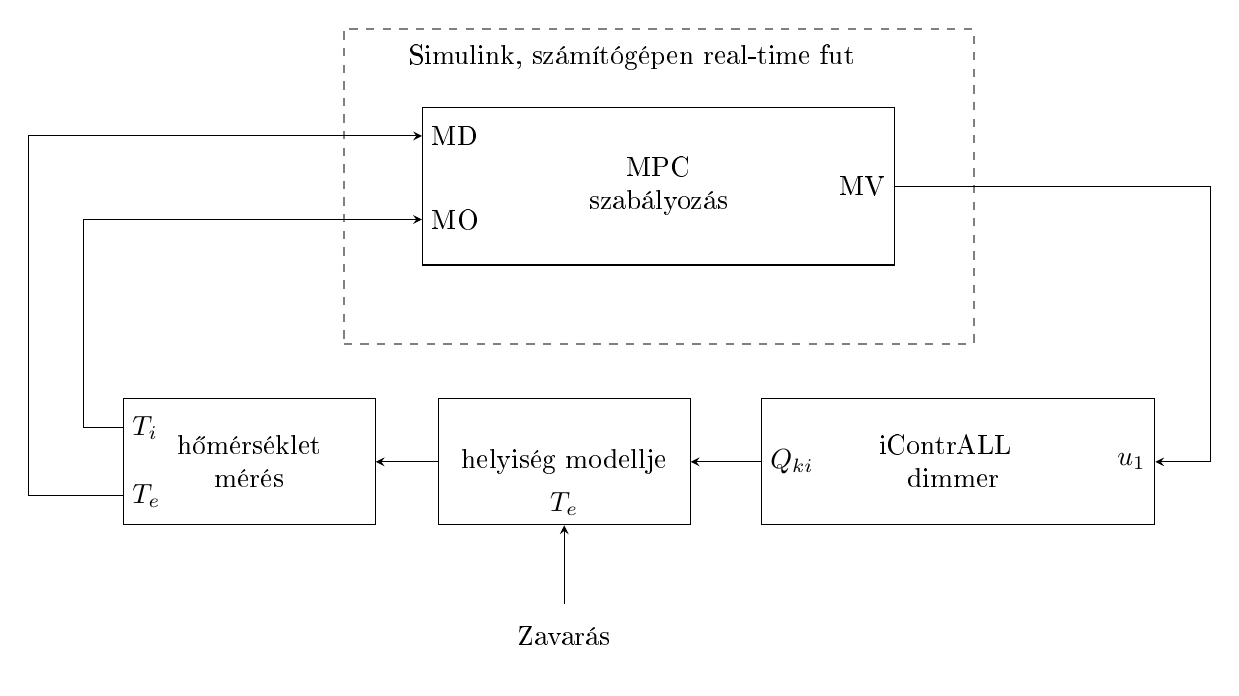
\begin{tikzpicture}[>=stealth,
  		%inner/.style={draw,fill=blue!5,thick,inner sep=3pt,minimum width=8em},
		%outer/.style={draw=gray,dashed,fill=green!1,thick,inner sep=5pt}
		outer/.style={draw=gray,dashed,thick,inner sep=5pt}
		]
	
	% Szabályzási kör elemei
	% ----------------------
	
		% Szabályzó
		\node[draw,rectangle, minimum height=2cm,minimum width=6cm] (MPC) at (3.2,3.5) {\parbox{2cm}{\centering MPC szabályozás}};		

		% Fűtési rendszer
		\node[draw,rectangle, minimum height=1.6cm,minimum width=5cm] (Heat) at (7,0) {\parbox{2cm}{\centering iContrALL~~~~ \\ dimmer~~}};
	
		% Ház
		\node[draw,rectangle, minimum height=1.6cm,minimum width=3.2cm] (House) at (2,0) {helyiség modellje};
		
		% Hőmérő
		\node[draw,rectangle, minimum height=1.6cm,minimum width=3.2cm] (Measure) at (-2,0) {\parbox{2cm}{\centering hőmérséklet\\mérés}};
		
		%Zavarás
		\node[rectangle, minimum height=0.8cm,minimum width=2cm,below=of House, node distance=1cm] (ghostDist)  {Zavarás};

		
	
	% Kiegészítő cuccok
	% ----------------------
	
	% Keret - Matlab
	\node[draw,outer,rectangle, minimum height=4cm,minimum width=8cm,
	label={[label distance=-0.1cm, anchor=north]100:Simulink, számítógépen real-time fut}] (keret) at (3.2,3.5) {};
	
	% Zavarás a modellbemenetre
	\draw[->] (ghostDist.90) --  (House.270) node[above]{$T_e$};
	
	%\draw[->] (ctr.191) node[right]{${u_{2}}$} -| ++(-1.7,1.3)|-  (Numeric.172) node[right]{$\alpha_{floor}$};  %node[above left]{$\alpha_{radiator}$}; 
	
	% mért változók
	\draw[->] (House.180) -- (Measure.0);
	\draw[->] (Measure.195) node[right]{$T_e$} -| ++(-1.2,0)  |-  (MPC.168) node[right]{MD} ;
	\draw[->] (Measure.165) node[right]{${T_{i}}$}-| ++(-0.5,0.8)  |-  (MPC.188) node[right]{MO} ;

	
	%\draw[->] (d.0) node[left]{heat [W]} ->  ++(3,0) ->  (house.180);
	% Beavatkozó jel
	\draw [->] (MPC.0) node[left]{MV} -| ++(4,-2.5)  |- (Heat.0) node[left]{${u_1}$}; %++(1.5cm,0) -- (2cm,0pt) -- (2.5cm,10pt);
	
	\draw[->] (Heat.180)  node[right]{$Q_{ki}$} -- (House.0) ;
	%\draw[->] (d.20) -| ++(1,-1) |- (y.350);
	
	%\path 
	%(d.150)	 edge[<->] 	node[anchor=north,above]{valvePercent}	(y.270);
	
	% Lehetséges label beállítások:
		%label={[blue,yshift=0.3cm]above:Z}]
	
%	\node[draw,outer,rectangle, minimum height=5.5cm,minimum width=13cm,
%	label={[label distance=-0.1cm, anchor=north]270:3 bemenetű, 1 kimenetű szakaszmodell}] (keret) at (0,15) {};
%	
%	
	\end{tikzpicture}

	\caption{A valós idejű mérések szereplői}
	\label{fig:realtimesimulink}
\end{figure}

%\begin{tikzpicture}[>=stealth,remember picture]
%\node[draw,rectangle,inner sep=0.5cm] (y) at (0,0) {$A$};
%\node[draw] (d) at (0,2) {%
%%	\begin{tikzpicture}[remember picture]
%%	\matrix [matrix of math nodes] (mat)
%%	{
%%		B & \phantom{C}   \\
%%		\phantom{B} & C \\
%%	};
%%	\end{tikzpicture}
%%};
%%\draw[->,shorten >= 6pt] (y.west) -| ++(-1,1) |- (mat-1-1);
%%\draw[->,shorten >= 6pt] (y.west) -| ++(-0.8,1) |- (mat-2-1);
%%\draw[->] ($(mat-2-2)+(14pt,0)$) -| ++(0.8,-1) |- (y.east);
%%\draw[->] ($(mat-1-2)+(14pt,0)$) -| ++(1,-1) |- (y.east);
%\end{tikzpicture}




% 3600001117-es ID-jű, Raspberry Pi, IP címe fixen 192.168.0.108, 54321-es port.

%A PI SPI-n küld a rádióadónak.
%Rádiókommunikáció egyirányú.

\section{Mintavételi idő és predikciós horizont}

Az MPC paraméterezésére \textit{Agachi \cite{romanMPC_Agachi}} könyvében találhatók ajánlások. A predikciós horizontot eszerint úgy kell megválasztani, hogy az a szakasz releváns dinamikáját lefedje. Mivel a felfutási ideje a kísérleti rendszernek kb. 1 óra, ezért ezt ekkorára választottam. A predikciós horizont ajánlott nagysága 10-20 mintavétel a számítási igény csökkentése miatt (így $T_s =$ \SI{300}{\second} adódna),  viszont a mérés során gyakrabban szerettem volna látni a változásokat, a mintavételi időt 30 másodpercnek vettem.

A fentiek mellett viszont a szabályzó nem adott ki beavatkozójelet egészen egy predikciós horizontnyi ideig, azaz majdnem 1 órán keresztül\footnote{Ha 300 másodperces mintavételi időt használtam és 10 mintányi predikciós horizontot, ugyanez volt a helyzet. Ez idő alatt az MPC valószínűleg az állapotbecslőjét inicializálja.}. Az MPC képes a költségfüggvényben figyelembe venni a predikciós horizonton belül a referenciajel jövőbeli változásait (ez a \textit{Signal Previewing}), ezt kipróbáltam annak érdekében, hogy ezt a \say{holtidőt} csökkentsem, ám ellentétes hatást értem el.

A Simulink blokk viszont támogatja az MPC-nek kezdeti érték megadását. A kezdeti érték nélküli MPC-t szimulációban (azaz nem valós időben) futtattam, majd leolvastam annak belső állapotát. Az \verb|mpcstate| függvénnyel létre kellett hoznom egy objektumot, ami a Simulinkben a szabályzót inicializálja. Ehhez szükség volt a szabályzó állapotteres szakaszmodelljének\footnote{Amikor az MPC-t létrehozzuk, a szakaszmodellt a Matlab állapotteressé alakítja.} becsült állapotára, a zavarjel becsült értékére, a zaj becsült értékére (ez esetben üres vektor), a legutóbbi beavatkozójelre és egy kovarianciamátrixra (ezt nullmátrixnak vettem).

Azzal, hogy a fenti objektumban a legutóbbi beavatkozójelet maximálisnak vettem, valós idejű futás esetén, a fizikai rendszer ugrásválaszánál nem kellett kivárnom egy órát, azaz a predikciós horizontnyi időt, hanem a szabályzó rögtön maximális beavatkozójelet adott ki.

%\begin{lstlisting}[
%style=Matlab-editor,
%basicstyle=\mlttfamily,
%escapechar=`,
%]
%mpcstate05=mpcstate(mpc_labsys05,[163 81.5 11600],-0.858,[],1,zeros(4))
%MPCSTATE object with fields
%Plant: [163 81.5000 11600]
%Disturbance: -0.8580
%Noise: [1×0 double]
%LastMove: 1
%MATLAB Command Window Page 2
%Covariance: [4×4 double]
%\end{lstlisting}

\section{Szabályozótervezés az identifikált modellre}

A valós idejű méréshez használt szabályzót érdemes először szimulációban megvizsgálni. Ekkor az identifikált lineáris modell a szabályzott szakasz, a szabályzóparaméterek megváltoztatását pedig gyorsan meg lehet figyelni.



\begin{figure}[H]
	\begin{subfigure}[t]{0.32\textwidth}
		\centering
		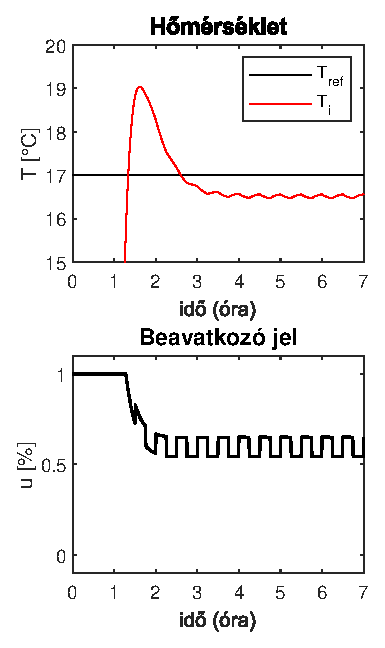
\includegraphics[width=\textwidth]{figures/realsys/mpc-wy-1}
		\caption{$w_y=1$}
		\label{fig:mpc-wy-1}
	\end{subfigure}
	~
	\begin{subfigure}[t]{0.32\textwidth}
		\centering
		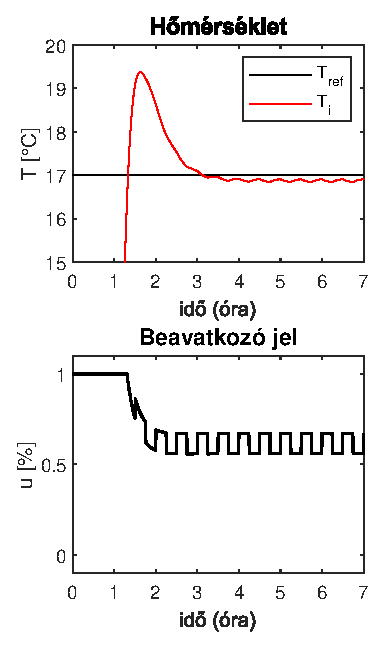
\includegraphics[width=\textwidth]{figures/realsys/mpc-wy-2}
		\caption{$w_y=2$}
		\label{fig:mpc-wy-2}
	\end{subfigure}
	~
	\begin{subfigure}[t]{0.32\textwidth}
		\centering
		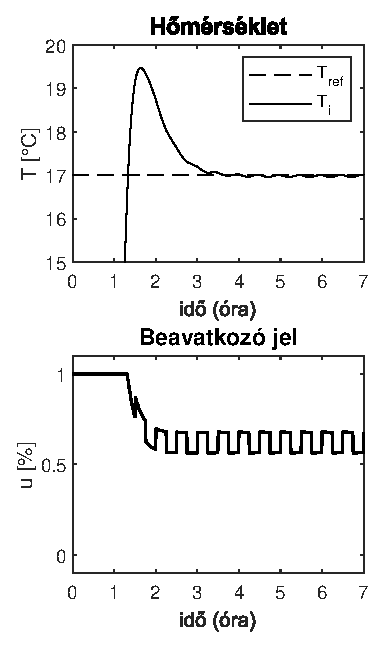
\includegraphics[width=\textwidth]{figures/realsys/mpc-wy-5}
		\caption{$w_y=5$}
		\label{fig:mpc-wy-5}
	\end{subfigure}
	\caption{MPC viselkedése különböző $w_y$ értékekre}
	\label{fig:mpc-wy}
\end{figure}



\begin{figure}[H]
\begin{subfigure}[t]{0.32\textwidth}
	\centering
	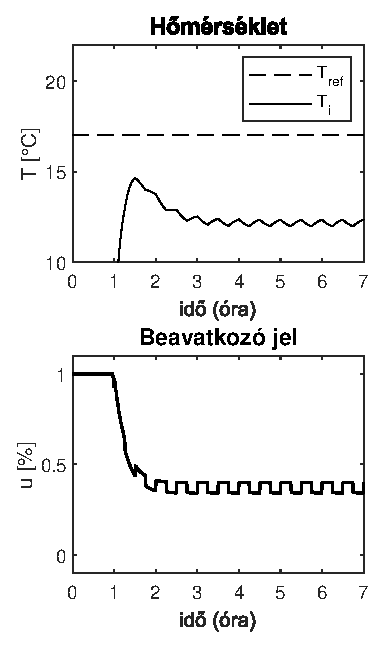
\includegraphics[width=\textwidth]{figures/realsys/mpc-wu-20}
	\caption{$w_u=20$}
	\label{fig:mpc-wu-20}
\end{subfigure}
~
\begin{subfigure}[t]{0.32\textwidth}
	\centering
	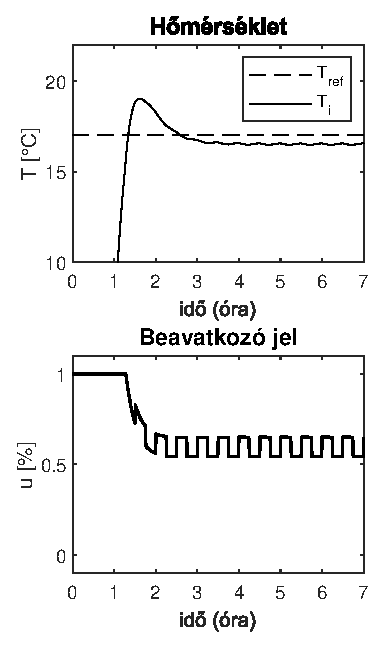
\includegraphics[width=\textwidth]{figures/realsys/mpc-wu-05}
	\caption{$w_u=5$}
	\label{fig:mpc-wu-05}
\end{subfigure}
~
\begin{subfigure}[t]{0.32\textwidth}
	\centering
	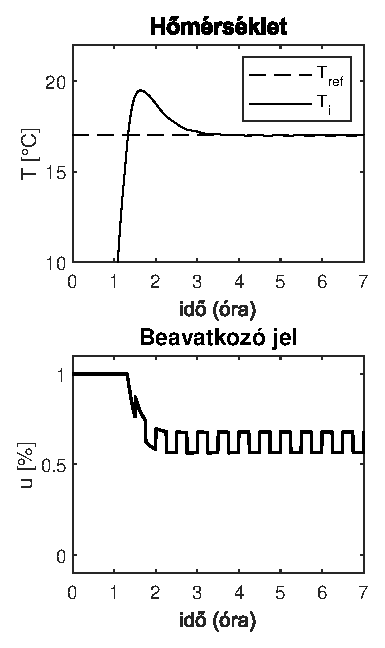
\includegraphics[width=\textwidth]{figures/realsys/mpc-wu-005}
	\caption{$w_u=0.05$}
	\label{fig:mpc-wu-005}
\end{subfigure}
\caption{MPC viselkedése különböző $w_u$ értékekre, $w_y=5$ mellett}
\label{fig:mpc-wu}
\end{figure}
\pagebreak

\begin{figure}[H]
\begin{subfigure}[t]{0.32\textwidth}
	\centering
	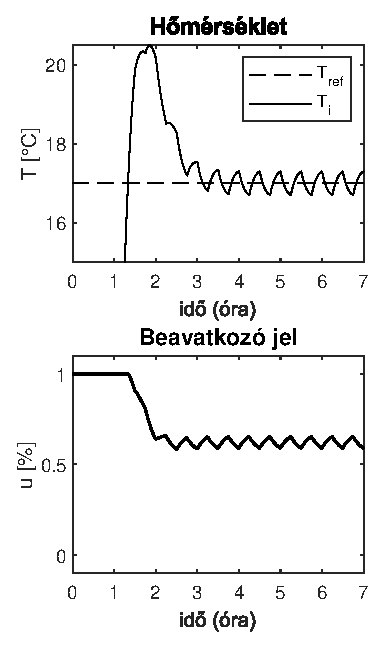
\includegraphics[width=\textwidth]{figures/realsys/mpc-wdu-100}
	\caption{$w_{\Delta u}=100$}
	\label{fig:mpc-wdu-100}
\end{subfigure}
~
\begin{subfigure}[t]{0.32\textwidth}
	\centering
	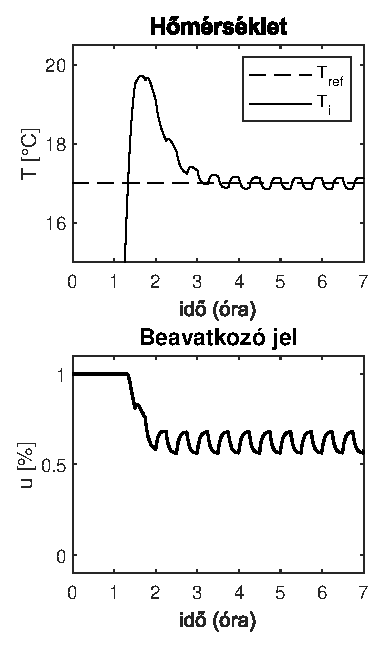
\includegraphics[width=\textwidth]{figures/realsys/mpc-wdu-50}
	\caption{$w_{\Delta u}=50$}
	\label{fig:mpc-wdu-50}
\end{subfigure}
~
\begin{subfigure}[t]{0.32\textwidth}
	\centering
	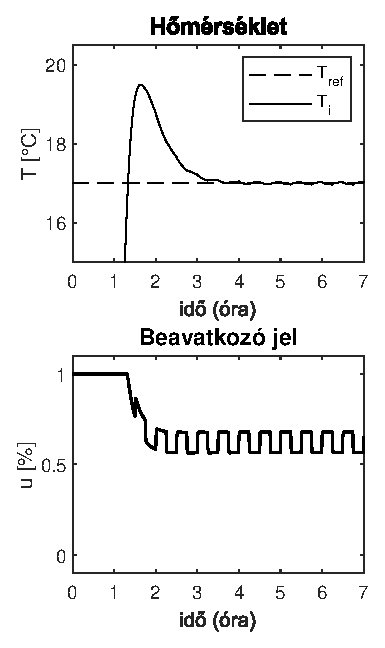
\includegraphics[width=\textwidth]{figures/realsys/mpc-wdu-10}
	\caption{$w_{\Delta u}=10$}
	\label{fig:mpc-wdu-10}
\end{subfigure}
\caption{MPC viselkedése  $w_{\Delta u}$ értékekre, $w_y=5$, $w_u=0.05$ mellett}
\label{fig:mpc-wdu}
\end{figure}





%% Feljesztési lehetőségek
%\begin{formal}
%	Még lehetséges:
%	\begin{itemize}[noitemsep,topsep=-8pt,parsep=0pt,partopsep=0pt]
%		%		\item kazán bekapcsolása
%		%		\item előremenő hőmérséklet - unmeasured VAGY uncontrolled inputként
%		%		\item 1 db. fűtőtest (most radiátor) szelepének tömegárama (szelep áteresztése)
%		%		\item Később több fűtőtest vagy többféle fűtőtestek (padlófűtés, különböző teljesítményű radiátorok) szabályozása
%		\item környezeti hőmérséklet: predikció / szekvencia használata% is lesz rá. Hatása a kimeneten már identifikálva lett, 3 pólussal és 2 zérussal tökéletesen lekövethető.
%		\item napsugárzás zavaró hatása% - szimulálható  a bizonytalansága valószínűleg nagy lesz
%	\end{itemize}
%	
%	Belső változók - fűtési rendszer és ház kapcsolata
%	\begin{itemize}[noitemsep,topsep=-6pt,parsep=0pt,partopsep=0pt]
%		\item napsugárzás - radiatív, az ablak felületével és a szöggel arányos
%		\item fűtőtestek sugárzó és konvektív hőárama
%	\end{itemize}
%	
%	Paraméterek a plantben nem állandók:
%	\begin{itemize}[noitemsep,topsep=-6pt,parsep=0pt,partopsep=0pt]
%		%		\item hőátadási tényezők hőmérsékletfüggők, áramlási sebesség-függők (szél)
%		\item szellőztetés, belső hőterhelés hatása
%	\end{itemize}
%\end{formal}
\chapter{Gyakorlati megvalósítás lehetőségei}

A szakdolgozatban vizsgált problémára adott elméleti megoldásnak számos dologi követelménye van, mivel vezérelhető szelepekkel, ismert paraméterekkel dolgozok. 

\section{Technikai feltételek}\label{chap:feasibility-tech}


\section{Piaci lehetőségek}

A következő részben személyes tapasztalatokat mutatok be, amelyek nem tükrözik a teljes piac helyzetét, részben akár a trendekkel ellentétesek is lehetnek. Azzal, hogy betekintést nyertem az építőipar egy szegletébe, jobban el tudtam képzelni, mi a fizikai tartalom a sok technológia mögött, amikkel az irodalomkutatás során találkoztam. Célom az volt, hogy képet szerezzek az alapvető elképzelésekről, elvárásokról egy HVAC rendszerrel szemben.

Egy nagy hazai kivitelező cég irodáinak látogatásakor figyeltem meg egy irodai környeztet. Arra voltam kíváncsi, adottak-e már a technikai feltételek egy ilyen szabályzás üzembe helyezéséhez, a konkrét irodában például az, hogy nagyobb átépítés nélkül\footnote{Azok a cégek, melyek azért építenek fel irodaházakat, hogy azokat bérbe adják, minél univerzálisabban szeretnének tervezni. Csak a központi magot, a szerkezeteket építik fel, a belsőépítészet, a \textit{héj} a bérlő igényei szerint valósul meg. Így előfordulhat, hogy bérlőcserekor átalakítják a bérlemény kinézetét, ekkor viszont alapvető épületgépészeti rendszerekhez nem nyúlnak hozzá.}, egy kész rendszerre is használható-e egy MPC szabályzás.

A meglátogatott épületben egy BMS (Building Management System) felügyelte a HVAC rendszereket. Ennek a géptermébe nem tudtam bemenni, de megfigyeltem az irodákban, a távhőközpontnál és a légkezelő egységeknél található gépészetet. A termosztátok Johnson Controls gyártmányúak voltak. Ez a cég gyártotta még az alkalmazott távhőszelepeket.

Az irodákban a HVAC tervezésébe nagy mértékben beleszólt a nagy belső hőterhelés, ami a zsúfolt irodában megjelenik: a tervezők radiátoros fűtés mellett döntöttek, ezeket Danfoss elektronikus szelepek vezérlik. (Azt nem tudom, hogy ezek kétállásúak-e vagy folytonosan szabályozhatóak, de előbbire gyanakszom.) Szobánként lettek termosztátok elhelyezve. A szellőztetésről és a hűtésről Lindab Professional klímagerendák gondozkodnak. A BMS feladata, hogy egyszerre a fűtés és a hűtés ne legyen bekapcsolva. Az egész rendszer tervezése - igaz a főépítésszel és nem az épületgépész munkatárssal beszéltem - során a költséghatékonyságra és az alacsony karbantartási költségre törekedtek.

%Külső árnyékolót sem használtak: korszerű ablakok használata mellett olyan alacsony a megtakarítás, hogy a megtérülési idő nagyon magas lett volna, illetve szélre érzékeny, karbantartást igénylő elem.
\chapter{További teendők, finomítások, lehetőségek}
\chapter{Összefoglalás}

%\cite{AFRAM2014343}


\pagebreak
\bibliographystyle{unsrt}
\bibliography{szakdogaforras}

%\bibliography{szakdogaforras}
%%\addcontentsline{toc}{chapter}{Irodalomjegyzék}
%\bibliographystyle{plain}

%\include{appendices}

\label{page:last}
\end{document}
